%%%%%%%%%%%%%%%%%%%%%%%%%%%
% PREAMBOLO DEL DOCUMENTO %
%%%%%%%%%%%%%%%%%%%%%%%%%%%
\documentclass[a4paper,11pt,oneside,top=3cm,bottom=3cm,left=3.5cm,right=3.5cm,openright,reqno,table]{book}
% openany - fa iniziare i capitoli direttamente nella pagina successiva
% openright - fa iniziare i capitoli nella prima pagina destra disponibile 
% fleqn  - allinea le formule a sinistra anzichè centrarle
% leqno - dispone la numerazione delle formule sulla sinistra o destra
% reqno - dispone la numerazione delle formule sulla destra
%
\usepackage{packages}
% Per non appesantire troppo questo file
% quasi tutti i pacchetti usati sono salvati in packages.sty
%
\linespread{1.5}
% Per avere la parola BOZZA scritta su tutte le pagine
%\usepackage[italian,first,light,bottomafter]{draftcopy}
\usepackage{array}
\usepackage{color}
\usepackage{colortbl}
% funziona solo in modalità PS
% Invece per i PDF ho risolto così:
% pdftk tesi.pdf background bozza.pdf output tesi_bozza.pdf
%
\renewcommand\lstlistingname{Algoritmo}
\renewcommand\lstlistlistingname{Elenco degli algoritmi}
\usepackage{float}
%%%%%%%%%%%%%%%%%%%%%%%%%%%%%%%%%
%   DOCUMENTO VERO E PROPRIO    %
%%%%%%%%%%%%%%%%%%%%%%%%%%%%%%%%%
\begin{document}
% FRONTESPIZIO %
\begin{titlepage}
\changepage{}{}{}{-7.5 mm}{}{}{}{}{}
% parametri per cambiare le dimensioni di una singola pagina in ordine:
% {textheight}{textwidth}{evensidemargin}{oddsidemargin}{columnsep}
% {topmargin}{headheight}{headsep}{footskip}
% se voglio centrare la pagina devo mettere bindingoffset/2
% i primi 5 parametri posso usarli con \changetext


\begin{center}

\includegraphics [width=.15\columnwidth, angle=0]{unisa}\\ % height
\vspace{0.5cm}
{\LARGE \scshape Universit\`{a} degli Studi di Salerno}\\
\vspace{0.5cm}
{\Large Dipartimento di Informatica}\\
\vspace{0.1cm}
{\large Corso di Laurea Triennale in Informatica}\\
\vspace{1.5cm}
{\Large \scshape Tesi di Laurea} \\
\vspace{4cm}
{\Huge \bfseries Visualizzazione di insiemi minimali di dipendenze funzionali rilassate} \\
\vspace{5cm}

\begin{minipage}[t]{7cm}
\flushleft
\textsc{Relatori}

Prof. \textbf{Vincenzo Deufemia} \\
Dott.ssa \textbf{Loredana Caruccio} \\
%{\small Universit\`{a} degli Studi di Salerno} \\[0.25cm]
\end{minipage}
\hfill
\begin{minipage}[t]{7cm}
\flushright
\textsc{Candidato}

\textbf{Giosu\`{e} Sulipano} \\
Matricola: 0512104715
\end{minipage}

\vspace{3cm}

{\small Anno Accademico 2018-2019} %\\
%
%
\begin{comment}
\begin{table}[!h]
\centering
\begin{tabular}{c c c} %p{5cm}c
& Tesi di laurea & \\
& \textbf{Giosuè Sulipano} & \\
& & \\[0.25cm]
Relatorei \\
Prof. \textbf{Vincenzo Deufemia} \\
Dott. \textbf{Loredana Caruccio} \\
{\small Università degli Studi di Salerno} & & {\small Provincia di Salerno}\\
& & \\[0.5cm]
& {\small A.A. 2018-2019} & \\
\end{tabular}
\end{table}
\end{comment}
%
%
\end{center}

\end{titlepage}
%

\frontmatter
% quello che segue è in numerazione romana e i capitoli non verranno numerati
% se non si vuole che compaia il numero di pagina basta usare il comando:
%\nonumber

% RINGRAZIAMENTI %
\begin{titlepage}

\nonumber
\null \vspace {\stretch{1}}
	\begin{flushright}
%	\begin{verse}
\textit{Ai miei genitori,\\per aver sempre creduto in me.} \\[5mm]
%RINGRAZIAMENTI
%	\end{verse}
	\end{flushright}



\end{titlepage}
% SOMMARIO %
\cleardoublepage
\selectlanguage{english}
\begin{abstract}
Le dipendenze tra dati rappresentano uno dei metadati chiave per caratterizzare e profilare sorgenti multimediali o in generale big data. Tuttavia, rispetto ai database tradizionali, in questi nuovi contesti \`{e} stato necessario introdurre alcune approssimazioni nella definizione delle dipendenze e ideare algoritmi di scoperta per estrarli automaticamente dai dati. Per il rilassamento delle dipendenze si mira ad effettuare un confronto approssimato ed a catturare dipendenze che non valgono sull'intero dataset. Ciononostante, le approssimazioni producono una proliferazione di dipendenze prodotte dagli algoritmi usati per il loro rilevamento, il che rende difficile per un utente analizzarle efficacemente. A tal fine, presentiamo un tool per classificare e visualizzare le dipendenze scoperte su big data, attraverso un grafico dinamico che permette di riassumere le dipendenze valide su un'istanza di database. In particolare, esso rappresenta la correlazione presente tra gli attributi, e come quest'ultima evolve al variare delle cardinalit\`{a} del lato sinistro delle dipendenze e delle soglie di confronto approssimato sia sul lato destro che sul lato sinistro delle dipendenze.
%\\[1cm]
\end{abstract}
\selectlanguage{italian}
% INDICI %
\phantomsection
\addcontentsline{toc}{chapter}{Indice}
\tableofcontents
% Il simbolo * serve per evitare che comapaia nell'indice
\clearpage
%\listoffigures
%\clearpage
%\listoftables
% GLOSSARIO
\cleardoublepage
\phantomsection
%\addcontentsline{toc}{chapter}{Glossario}
% per inserire l'elenco dei simboli e degli acronimi nell'indice

\newacronym{fd}{FD}{Dipendenza Funzionale}
\newacronym{fds}{FD}{Dipendenze Funzionali}
\newacronym{rfd}{RFD}{Dipendenza Funzionale Rilassata}
\newacronym{rfds}{RFD}{Dipendenze Funzionali Rilassate}

\printglossary
% Per stampare il glossario

% per aggiornarlo si deve eseguire da terminale:
% makeindex -s myDoc.ist -t myDoc.alg -o myDoc.acr myDoc.acn
% per inserire una voce nell'elenco:
% \newglossaryentry{voce_etichetta}{name={voce}, description={descrizione}}
% se non compare direttamente nel testo va inizializzata con:
% \glsadd{voce_etichetta}
% oppure se viene richiamata all'interno del testo:
% \gls{voce_etichetta}
% SIMBOLI E NOTAZIONI %
\cleardoublepage
\phantomsection
\addcontentsline{toc}{chapter}{Elenco delle figure}
% per inserire l'elenco dei simboli e degli acronimi nell'indice
%\printglossary[type=\acronymtype,title=Elenco delle figure]
% Per stampare l'elenco dei simboli
\listoffigures
\cleardoublepage
\phantomsection
\addcontentsline{toc}{chapter}{Elenco delle tabelle}
% per inserire l'elenco dei simboli e degli acronimi nell'indice
%\printglossary[type=\acronymtype,title=Elenco delle figure]
% Per stampare l'elenco dei simboli
\listoftables
\cleardoublepage
\phantomsection
\addcontentsline{toc}{chapter}{Elenco dei listings}
% per inserire l'elenco dei simboli e degli acronimi nell'indice
%\printglossary[type=\acronymtype,title=Elenco delle figure]
% Per stampare l'elenco dei simboli
\lstlistoflistings
% per aggiornarlo si deve eseguire da terminale:
% makeindex -s myDoc.ist -t myDoc.glg -o myDoc.gls myDoc.glo
% per inserire una voce nell'elenco:
% \newglossaryentry{voce_etichetta}{name={voce}, description={descrizione}}
% se non compare direttamente nel testo va inizializzata con:
% \glsadd{voce_etichetta}
% oppure se viene richiamata all'interno del testo:
% \gls{voce_etichetta}

\mainmatter
% quello che segue sarà in numerazione araba e i capitoli verranno numerati
%\part{Studio iniziale}
% CAPITOLI
\phantomsection
%\addcontentsline{toc}{chapter}{Introduzione}
\chapter{Introduzione}
\markboth{Introduzione}{}
% [titolo ridotto se non ci dovesse stare] {titolo completo}

\section{Motivazioni e Obiettivi} %\label{1sec:scopo}
L'evoluzione da dati tradizionali a dati complessi (e.g., multimediali, geografici e fuzzy) e successivamente ai big data, ha sollevato la necessit\`{a} di progettare metodi e strumenti per estrarre automaticamente e visualizzare le informazioni e statistiche da questi. Queste statistiche includono le classificazioni, le regole di associazione e diversi tipi di metadata \cite{profiling-relational-data}, come i value patterns, le foreign keys e le dipendenze dei dati, del tipo multivalore, inclusione e \acrlong{fds} (\acrshort{fds}) \cite{surveydatabasedependency}. Queste ultime venivano usate principalmente nei tradizionali database alfanumerici a scopi di normalizzazione\footnote{La \textbf{normalizzazione} \`{e} un processo atto ad eliminare le ridondanze ed il rischio di incoerenza dal database.}. Successivamente, con l'evoluzione delle tecnologie alla base dei database, nuovi tipi di \acrlong{fds} sono state definite, come ad esempio le Dipendenze Funzionali Fuzzy \cite{ffdandlljoin} e le Dipendenze Multimediali \cite{nomalizationframework}, le quali introducono alcune approssimazioni necessarie per confrontare dati complessi, ma anche per tener conto dei confronti testuali, dei valori mancanti, delle dipendenze parzialmente valide ed altre approssimazioni nel contesto di applicazioni per big data. A tal fine, sono state introdotte oltre trenta definizioni differenti di Dipendenze Approssimate, chiamate anche \acrlong{rfds} (\acrshort{rfds}) \cite{rfdsurvey}. Nel contesto dei big data, le \acrlong{rfds} insieme ad altri metadati di profilazione sono utilizzate per diversi scopi, tra cui pulizia dei dati, ottimizzazione delle query e cos\`{i} via. Tuttavia, in questo contesto potrebbe essere difficile specificare le \acrlong{rfds} in fase di progettazione, insieme ai parametri che definiscono il loro livello di approssimazione, come ad esempio la similitudine tra valori di attributi e le soglie per indicare la porzione di dataset su cui una \acrlong{rfd} risiede. Quindi, \`{e} stato necessario escogitare metodi per la ricerca automatica delle \acrlong{rfds} nei dati \cite{ddiscoveryfromdata}. La ricerca delle \acrlong{rfds} nei dati \`{e} possibile grazie alla disponibilit\`{a} di raccolte di big data, poich\'{e} forniscono un'elevata rilevanza statistica per dipendenze approssimative che altrimenti dovrebbero essere specificate in fase di progettazione, in base alla semantica dei dati. D'altro canto, sorgono due problemi principali con gli algoritmi di scoperta di \acrlong{rfds} applicati ai big data:
\begin{enumerate}
    \item complessit\`{a} computazionale,
    \item visualizzazione dei risultati.
\end{enumerate}
Il primo \`{e} un problema gi\`{a} sufficientemente complesso anche con le \acrlong{fds} tradizionali e la sua complessit\`{a} cresce considerabilmente con l'introduzione delle approssimazioni, specialmente quando il numero di attributi cresce. Il secondo problema riguarda la complessit\`{a} dei risultati, perch\'{e} gli algortimi di ricerca delle \acrlong{rfds} spesso restituiscono in output un enorme set di dipendenze, con molte combinazioni di soglie differenti, il che rende difficile per un utente ricavare informazioni utili da queste. Ad oggi non \`{e} stato fornito alcun metodo di visualizzazione per le \acrlong{rfds}. L'obiettivo, quindi, \`{e} quello di progettare uno strumento che faciliti l'individuazione e la lettura delle informazioni utili riguardanti le \acrlong{rfds}. La tecnica di visualizzazione da utilizzare si applica alle \acrlong{rfds} scoperte da dati multimediali e big data e rappresenta sia le dipendenze scovate sia le loro soglie, includendo una strategia di classificazione che mira a selezionare le \acrlong{rfds} pi\`{u} rilevanti e significative su un determinato dataset.

\section{Risultati}
\begin{figure}[ht]
    \centering
    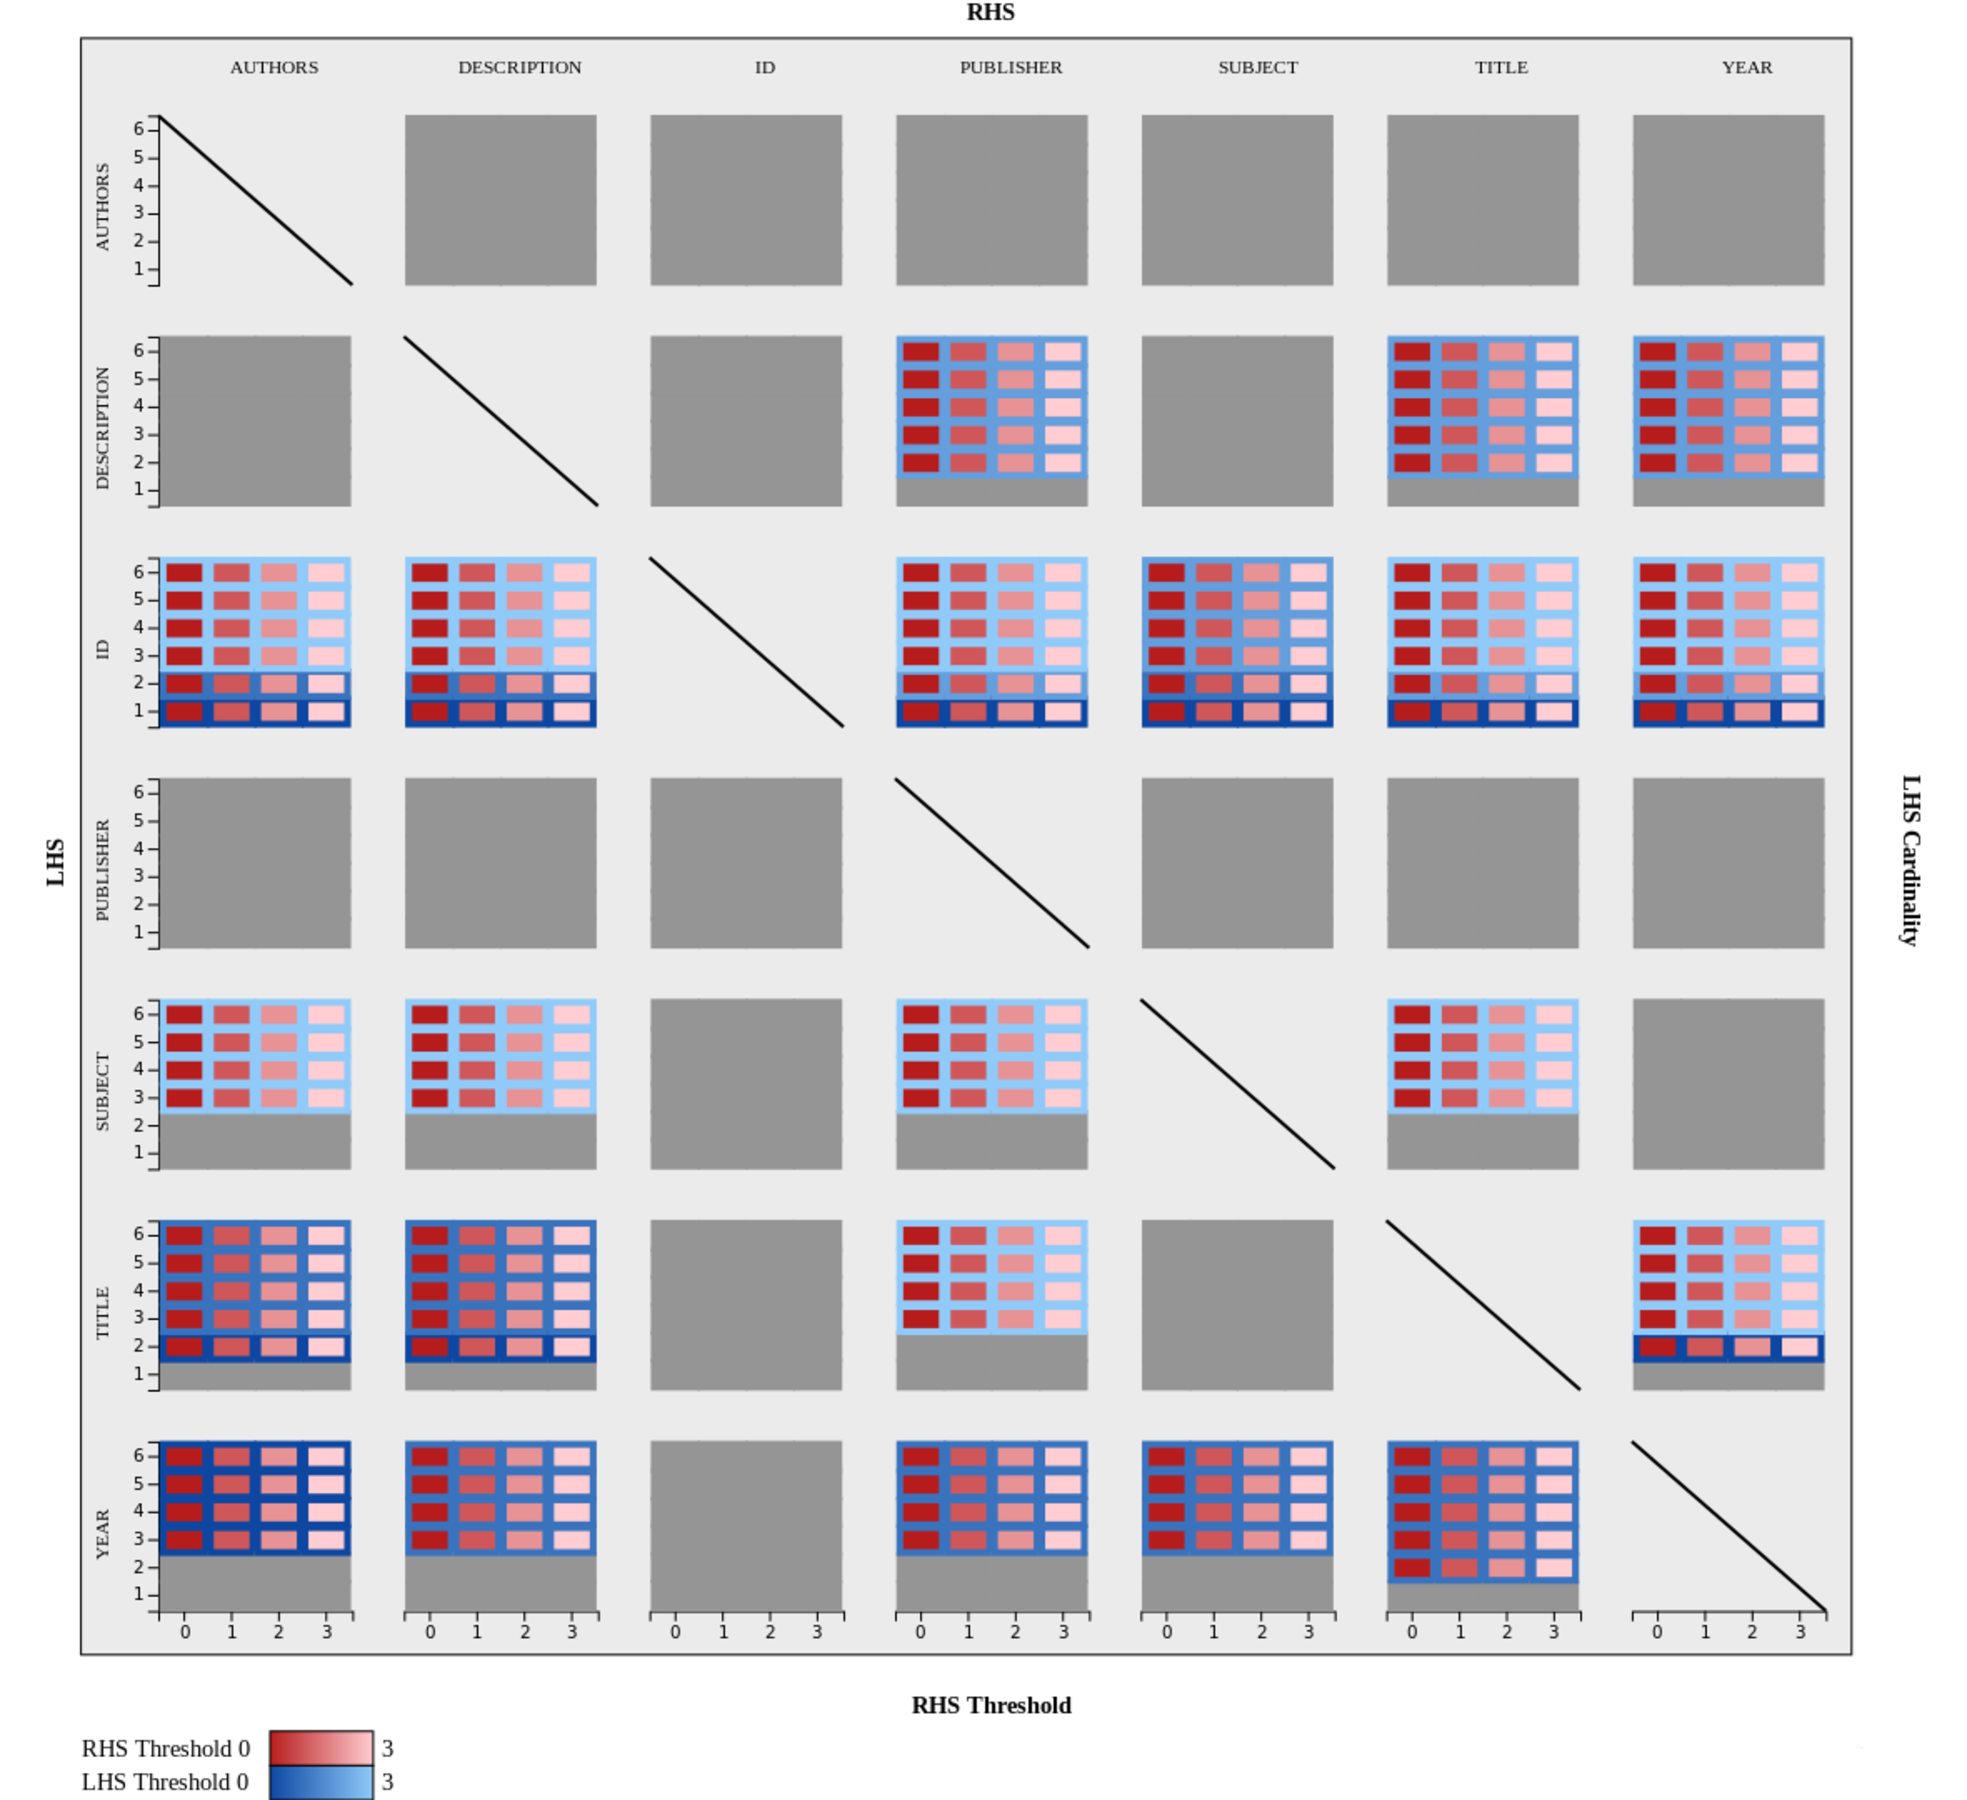
\includegraphics[width=\linewidth]{capitoli/figure/citiseer_2000_result}
    \caption{Rappresentazione ottenuta in output da Dependensee del dataset Citiseer 2000.}
    \label{fig:citiseer_2000_result}
\end{figure}
\begin{figure}[ht]
    \centering
    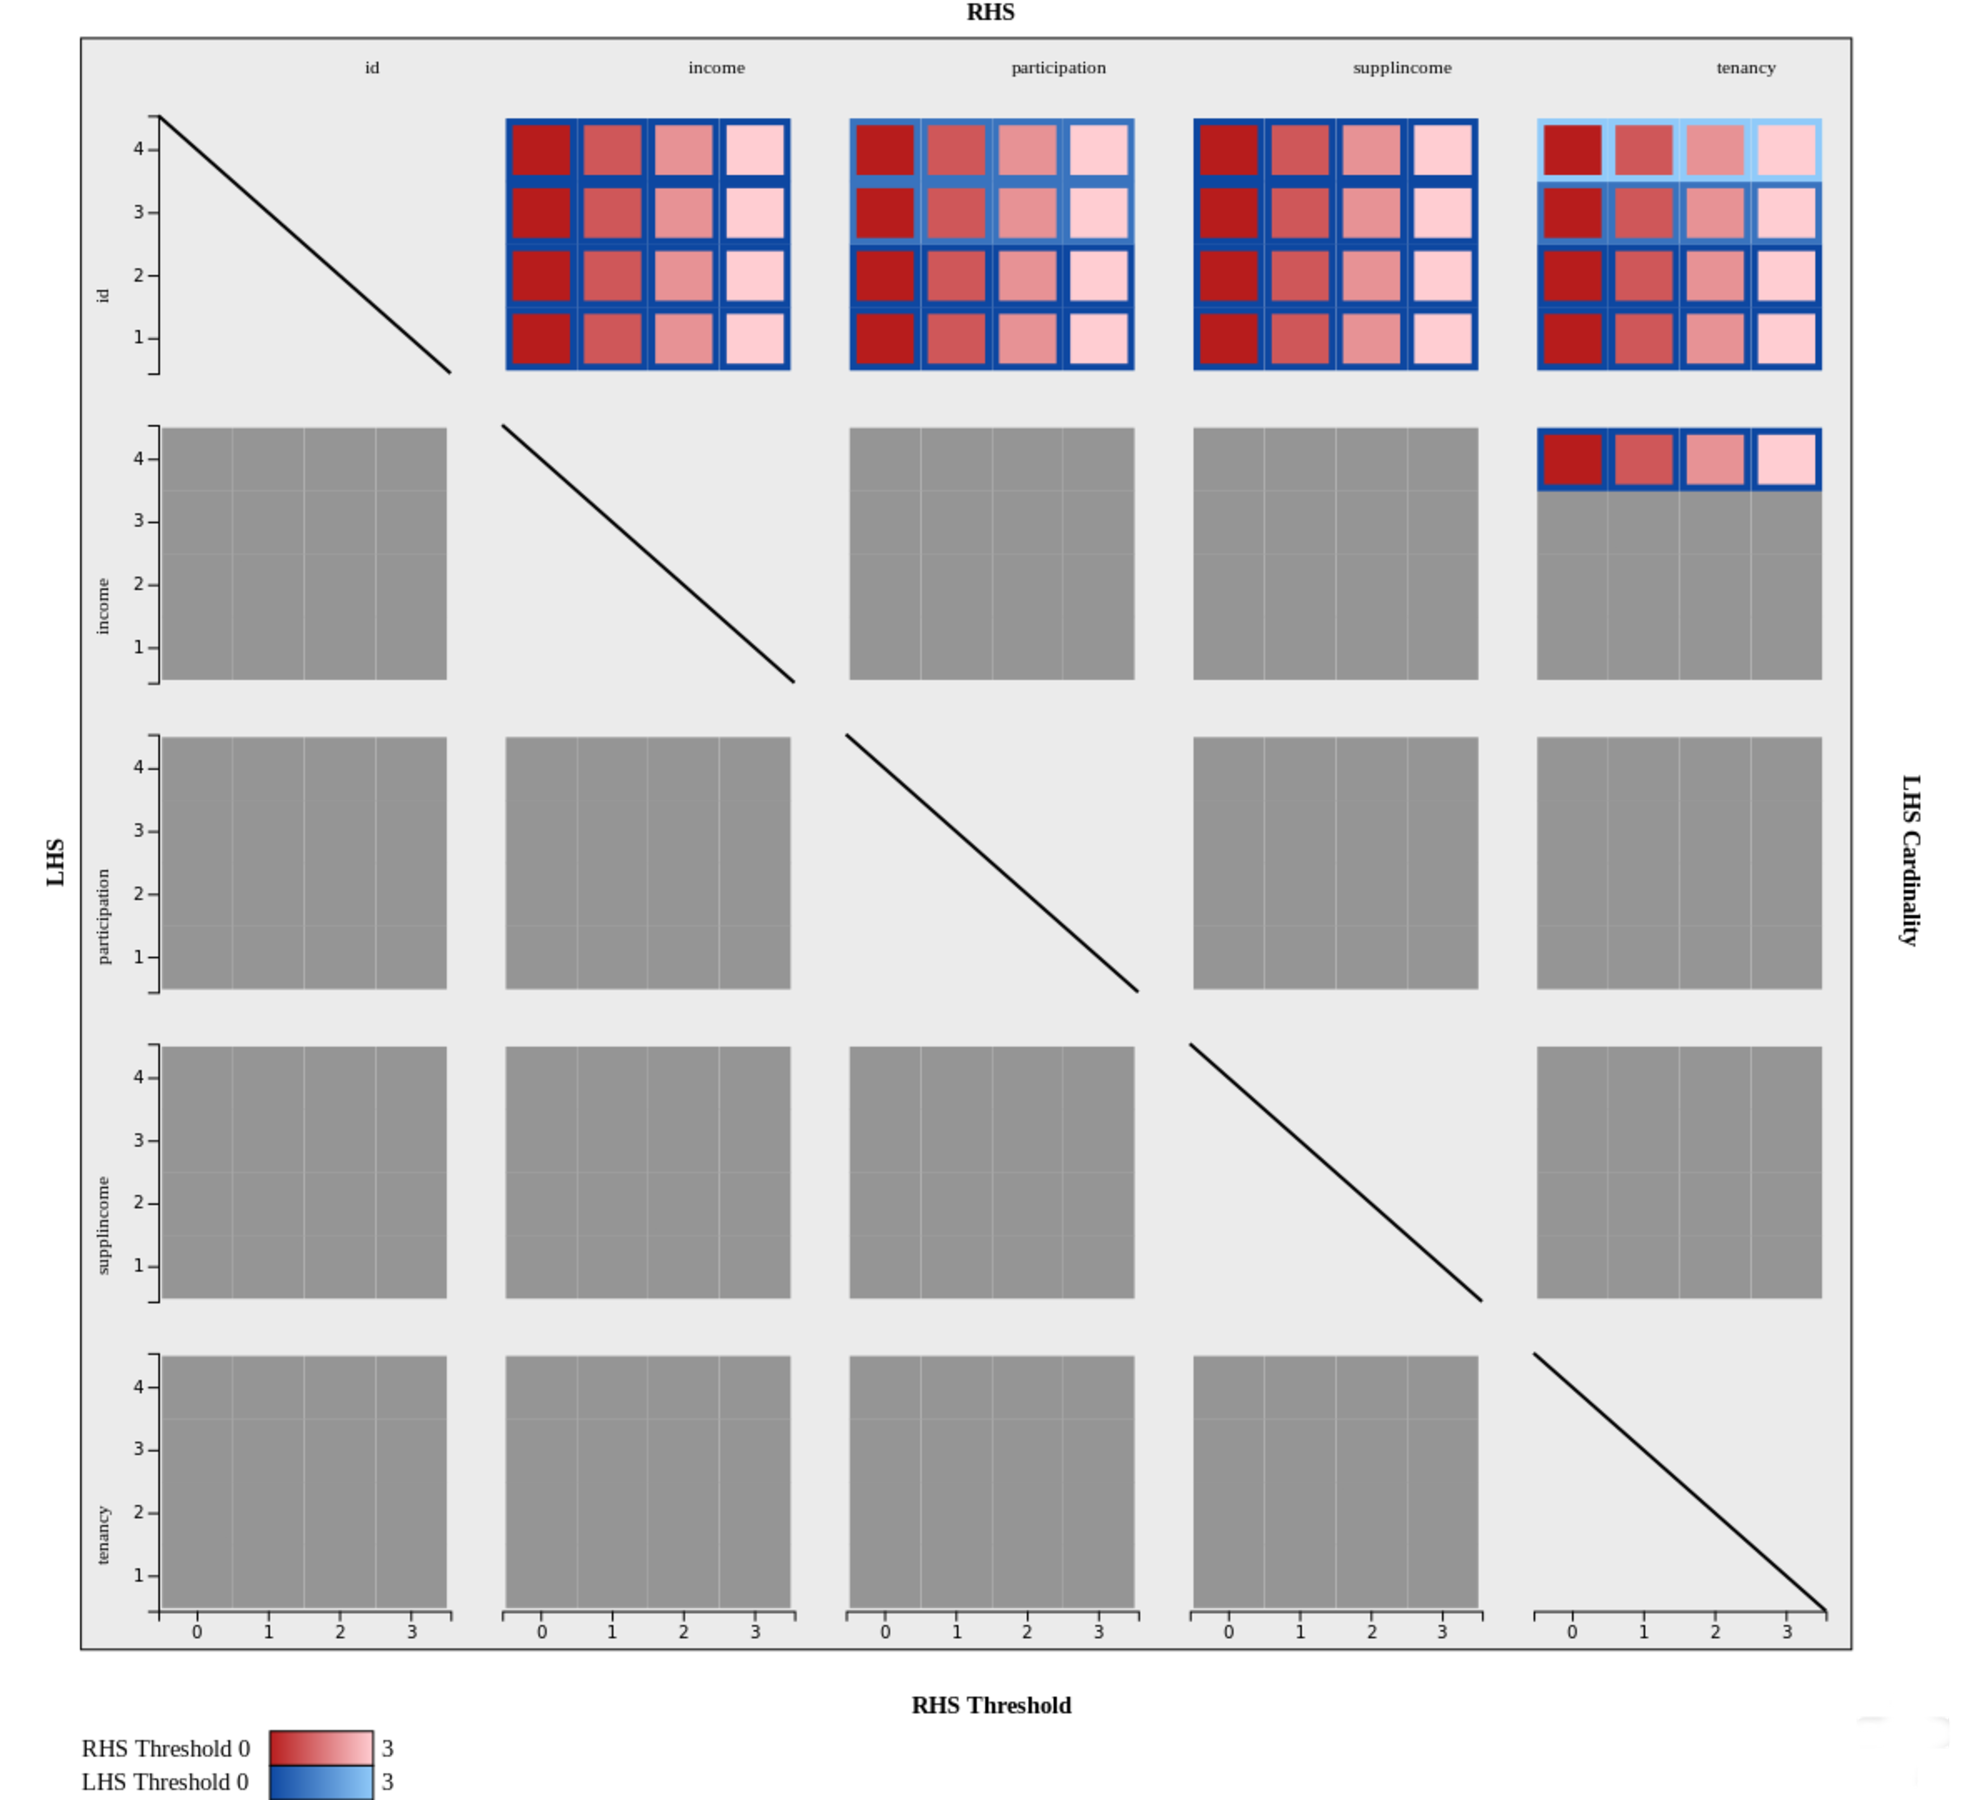
\includegraphics[width=\linewidth]{capitoli/figure/foodstamp_result}
    \caption{Rappresentazione ottenuta in output da Dependensee del dataset Foodstamp.}
    \label{fig:foodstamp_result}
\end{figure}
Attraverso l'implementazione della metafora di visualizzazione esposta nel capitolo \ref{section:visual_rep_metaphore} all'interno di Dependensee\footnote{\textbf{Dependensee} \`{e} il tool proposto per ovviare al problema dell'analisi visiva delle \acrshort{rfds} minimali.}, si \`{e} riusciti a rappresentare in modo immediato ed efficace un dataset di \acrlong{rfds}. In questo modo \`{e} stato possibile effettuare un'analisi visiva quasi istantanea, grazie alle diverse caratteristiche messe in luce dalla rappresentazione grafica fornita dallo strumento. Infatti, questa rappresentazione raffigura le dipendenze minimali esistenti tra tutti gli attributi contenute nel dataset, mettendo in risalto la cardinalit\`{a} del lato sinistro e le thresholds associate sia per il lato sinistro che per il lato destro.\par
La Figura \ref{fig:citiseer_2000_result} mostra la rappresentazione grafica ottenuta analizzando il dataset \textit{Citiseer 2000} con il tool proposto. Da un primo sguardo si pu\`{o} notare come questa faciliti effettivamente l'analisi visiva per l'utente. Analizzando il dataset attraverso tale rappresentazione possiamo notare, mediante la diagonale nulla, come le \acrfull{rfds} banali non vengano rappresentate. Se prendiamo in considerazione la prima riga, possiamo notare come non esistano \acrfull{rfds} minimali con l'attributo \texttt{AUTHORS} sul lato sinistro e con almeno un attributo diverso sul lato destro. Mentre, con la colonna relativa all'attributo \texttt{ID}, possiamo notare l'assenza di \acrfull{rfds} minimali con l'attributo relativo sul lato destro. Se analizziamo la sotto-matrice relativa all'attributo riga \texttt{TITLE} ed all'attributo colonna \texttt{AUTHORS}, possiamo notare l'assenza di \acrfull{rfds} con cardinalit\`{a} pari a 1 e l'esistenza di \acrfull{rfds} minimali con threshold pari a 0 sul lato sinistro e cardinalit\`{a} pari a 2, mentre per cardinalit\`{a} maggiori vi sono \acrfull{rfds} con threshold diverse da 0 ma con valori vicini a questo.\par
Consideriamo adesso il dataset \textit{Foodstamp}. La Figura \ref{fig:foodstamp_result} mostra la rappresentazione grafica ottenuta dando in input il dataset a Dependensee, il tool proposto. Dal grafico ottenuto possiamo notare, attraverso la prima riga, come le uniche dipendenze esistenti siano con l'attributo \texttt{id} sul lato sinistro e, attraverso la seconda riga, con l'attributo \texttt{income} sul lato sinistro. Le prime sono in relazione con tutti gli altri attributi del dataset, infatti le colonne relative alla prima riga sono tutte colorate. Mentre, per l'attributo \texttt{income}, possiamo notare l'esistenza di \acrfull{rfds} solo con l'attributo \texttt{tenancy} sul lato destro. Con le righe e le colonne restanti possiamo notare che non vi sono \acrfull{rfds}, difatti sono colorate in grigio.

\section{Struttura della tesi}
La tesi \`{e} strutturata come segue. Il capitolo \ref{cap2:stato_arte} esamina gli approcci esistenti in letteratura per visualizzare i metadati estratti dai big data. Il capitolo \ref{cap3:fd} fornisce alcune definizioni di background sulle \acrfull{rfds} ed una breve introduzione sugli algoritmi per la loro estrazione dai dati. Il capitolo \ref{cap4:visual_representation} introduce il concetto di minimalit\`{a} per filtrare le \acrfull{rfds} rilevanti ed una metafora di visualizzazione per rappresentare tali dipendenze. Il capitolo \ref{cap5:dependensee} introduce \textit{Dependensee}, il tool sviluppato durante il lavoro di tesi per la visualizzazione di insiemi minimali di \acrfull{rfds}.
\chapter{Stato dell'arte}%\label{1cap:spinta_laterale}
\label{cap2:stato_arte}
% [titolo ridotto se non ci dovesse stare] {titolo completo}
%

%\begin{citazione}
Questo capitolo illustra lo stato dell'arte e i lavori presenti in letteratura sugli aspetti di ricerca trattati nel nostro studio. Il problema della visualizzazione di grandi insiemi di \acrshort{rfds} automaticamente estratte dai dati \`{e} un problema recente. Ci\`{o} \`{e} dovuto ai recenti miglioramenti delle prestazioni degli algoritmi per l'estrazione delle \acrshort{rfds} dai dati e al potenziale delle soluzioni parallele che consentono la loro scoperta dai big data. Quindi, \`{e} sorto solo di recente il problema della gestione di grandi insiemi di \acrshort{rfds}, molti dei quali differiscono solo per il valore delle soglie di approssimazione. Per questo motivo, nella letteratura non vi sono soluzioni proproste per gestire tale complessit\`{e}, n\'{e} in termini di ranking e riepilogo delle \acrshort{rfds} trovate, n\'{e} in termini di tecniche di visualizzazione.\par
Gran parte del lavoro \`{e} stato svolto nell'ambito delle tecniche di visualizzazione dei dati e dei metadati \cite{topicmodeling}. Comunque, nel contesto di visualizzazione dei metadati \`{e} stata posta poca attenzione alla visualizzazione delle dipendenze. Un tentativo in questa direzione \`{e} stato fatto nel \cite{frameworktoanalyzeinfo}, dove oltre a fornire una tecnica per visualizzare le \acrshort{fds}, il concetto stesso di \acrshort{fd} viene sfruttato per visualizzare altre caratteristiche dei dati. In particolare, gli autori definiscono lo schema di visualizzazione funzionale, il quale rappresenta una mappatura visiva come un insieme di \acrshort{fds} tra dati e attributi visivi.\par
Un'altra proposta interessante \`{e} il progetto Metanome \cite{dataprofilingwithmetanome}, che \`{e} una piattaforma che include diversi algoritmi per la ricerca automatica di metadati complessi, includendo dipendenze funzionali e di inclusione. Per facilitarne l'analisi, Metanome offre diverse metriche di ranking, insieme a tecniche di visualizzazione per \acrshort{fds} e dipendenze di inclusione.\par
Tra gli approcci correlati alla visualizzazione delle dipendenze, vale la pena menzionare quelli che puntano alla visualizzazione delle regole associative (ARs) \cite{chenvisualanalysis,visualassrules,wifisviz,assocexplorer}. Infatti, il concetto di AR \`{e} in qualche modo correlato a quello di \acrshort{rfd}. In particolare, sebbene una AR rappresenti co-occorrenze di valori piuttosto che una correlazione di un attributo, il formalismo usato per rappresentare le \acrshort{rfds} e le ARs \`{e} simile e possono essere visualizzate utilizzando una metafora comune. Inoltre, le AR incorporano il concetto di confidence che \`{e} altamente correlato al concetto di estensione delle \acrshort{rfds}. Tra i metodi di visualizzazione per rappresentare le ARs vale la pena menzionare il mosaic plot \cite{visualassrules}, lo scatter plot \cite{assocexplorer}, il node-link graph \cite{wifisviz} ed il matrix \cite{vaet}. Il tool ARVis fu proposto per validare ed esplorare ARs, mentre il tool in \cite{visualassrulesusingmatrix} fornisce pi\`{u} viste per ispezionare visivamente l'insieme generale di AR. Infine, \`{e} stata presentata una tecnica di visualizzazione basata su matrice gerarchica in \cite{chenvisualanalysis}, dove gli autori forniscono un'organizzazione gerarchica delle loro matrici per migliorare l'esplorazione e la visualizzazione delle ARs.\par
Come accennato in precedenza, la situazione per le \acrshort{rfds} \`{e} molto pi\`{u} complessa, poich\'{e} rispetto alle \acrshort{fds}, gli algoritmi di ricerca per le \acrshort{rfds} potrebbero produrre in output molte pi\`{u} dipendenze, molte delle quali potrebbero avere lievi differenze nelle soglie di similitudine o di coverage. Questo aumenta enormemente la necessit\`{a} di escogitare metodi di visualizzazione e di ranking per permettere all'utente un'analisi rapida dei risultati dei processi di ricerca delle \acrshort{rfds} e migliorare i processi decisionali basati su di essi. Date le caratteristiche differenti delle \acrshort{rfds} rispetto alle \acrshort{fds}, le tecniche di visualizzazione e di ranking attualmente disponibili per le \acrshort{fds} non sono adatte ai nostri obiettivi, n\'{e} sono facilmente adattabili per visualizzare aspetti peculiari delle \acrshort{rfds}, come le soglie di similudine e di coverage.
%\end{citazione}

\newpage
\phantomsection
%\addcontentsline{toc}{chapter}{Dipendenze Funzionali per Big Data e Dati Multimediali}
\chapter{Dipendenze Funzionali per Big Data}
\label{cap3:fd}
\markboth{Dipendenze Funzionali per Big Data}{}
% [titolo ridotto se non ci dovesse stare] {titolo completo}
In questo capitolo verr\`{a} introdotto il concetto di \acrlong{rfd} per big data. Sebbene tali database possano essere organizzati in modo pi\'{u} adeguato mediante modelli di dati flessibili, come ad esempio NoSQL, nel seguito faremo riferimento al modello di dati relazionale, per motivi di semplicit\`{a}, rigore delle definizioni e senza perdita di generalit\`{a}.\par
Di seguito l'acronimo \acrshort{fd} verr\`{a} utilizzato per indicare le \acrlong{fds} e \acrshort{rfd} verr\`{a} utilizzato per indicare le \acrlong{rfds}.

\section{Concetti Preliminari} %\label{1sec:scopo}
Si consideri uno schema di database relazionale $\mathcal{R}$ definito su un insieme di attributi $attr(\mathcal{R})$, derivato come unione degli attributi degli schemi di relazione che compongono $\mathcal{R}$. Per un'istanza $r$ in $\mathcal{R}$, un attributo $A \in attr(\mathcal{R})$ ed una tupla $t \in r$, utilizziamo $t[A]$ per denotare la proiezione di $t$ su $A$; allo stesso modo, per un insieme $X$ di attributi in $attr(\mathcal{R})$, $t[X]$ denota la prezione di $t$ su $X$. Una \acrshort{fd} su $\mathcal{R}$ \`{e} una dichiarazione $X \rightarrow Y$ ($X$ implica $Y$), con $X, Y \subseteq attr(\mathcal{R})$, tale che, data un'istanza $r$ di $\mathcal{R}$, $X \rightarrow Y$ \`{e} soddisfatta in $r$ se e soltanto se per ogni coppia di tuple $(t_1, t_2)$ in $r$, tutte le volte che $t_1[X]=t_2[X]$, allora $t_1[Y]=t_2[Y]$.\par
Dalla definizione precedente possiamo notare come le proiezioni di due tuple, su un insieme di attributi, vengano confrontate mediante una funzione di uguaglianza. Ci\`{o} non \`{e} possibile in un contesto di big data o dati multimediali. Ad esempio, nel contesto dei dati multimediali \`{e} inconcepibile confrontare immagini o suoni mediante paradigmi di esatta corrispondenza. Piuttosto, potrebbero essere confrontate mediante funzioni di somiglianza che per le immagini potrebbero basarsi su attributi come colore, texture, forma e cos\`{i} via, mentre per i suoni potrebbero basarsi su volume, tono, larghezza di banda e cos\`{i} via. Considerazioni simili possono essere effettuate per i big data, nel caso di dati alfanumerici potrebbero essere necessari dei confronti approssimati a causa dei differenti formati, errori nei dati, inconsistenze e scale diverse. Inoltre, in ambo i contesti di big data e multimedia, potrebbero esserci dipendenze rilevanti che sono valide solo su un sottoinsieme di dati. Per questa ragione, la definizione di \acrshort{fd} \`{e} stata estesa in diversi modi per considerare i confronti approssimati tra tuple e misure per specificare il sottoinsieme di dati su cui una data dipendenza si applica. A tal fine, molte nuove definizioni fanno affidamento ai valori soglia per valutare la somiglianza nei confronti tra coppie di tuple o per specificare il numero minimo di tuple a cui una dipendenza deve applicarsi per essere valida.

\section{Dipendenze Funzionali Rilassate}
\theoremstyle{definition}
\newtheorem{rfddef}{Dipendenze funzionali rilassate}
\begin{rfddef}\label{def:rfd}
Si consideri uno schema di database relazionale $\mathcal{R}$ ed uno schema di relazione $R = (A_1, A_2,\text{\textellipsis}, A_m)$ di $\mathcal{R}$. Una \acrshort{rfd} $\varphi$ su $\mathcal{R}$ \`{e} indicata da
\begin{equation}
    \mathbb{D}_c : X_{\Phi1} \xrightarrow{\Psi\leq\varepsilon} Y_{\Phi_2}
\end{equation}
dove:
\begin{itemize}
    \item $\mathbb{D}_c=\{t \in dom(R) | \bigwedge\limits_{\imath=1}^{m}c_{\imath}(t[A_{\imath}])\}$
    \\con $c=(c_1,\text{\textellipsis},c_m)$ ed ogni $c_\imath$ \`{e} un predicato su $dom(A_\imath)$ che filtra le tuple su cui $\varphi$ si applica;
    \item $X=X_1,\text{\textellipsis},X_h \text{ e } Y=Y_1,\text{\textellipsis},Y_k$, con $X,Y\subseteq attr(R)$ e $X\cap Y=\emptyset$;
    \item $\Phi_1=\bigwedge\limits_{X_\imath \in X}\phi_\imath[X_\imath] \text{ (} \Phi_2=\bigwedge\limits_{Y_\jmath \in Y}\phi_\jmath[Y_\jmath] \text{, analog.)}$, dove $\phi_\imath \text{ (}\phi_\jmath\text{, analog.)}$ \`{e} un vincolo su $X_\imath$ ($Y_\jmath$, analog.) con $\imath=1,\text{\textellipsis},h$ ($\jmath=1,\text{\textellipsis},k$, analog.). Ogni $\phi_\imath$ \`{e} un predicato che coinvolge una funzione di distanza o similitudine, definita sul dominio di $X_\imath$, pi\`{u} uno o pi\`{u} operatori di confronto con soglie associate. Per ogni coppia di tuple $(t_1,t_2)\in\mathbb{D}_c$, il vincolo $\Phi_1$ ($\Phi_2$, analog.) \`{e} vero se la similitudine o la distanza tra $t_1[X_\imath]$ e $t_2[X_\imath]$ ($t_1[Y_\jmath]$ e $t_2[Y_\jmath]$, analog.) soddisfa il vincolo $\phi_\imath$ ($\phi_\jmath$, analog.) $\forall \imath \in [1,h]$ ($\jmath \in [1,k]$, analog.);
    \item $\Psi$ \`{e} una misura di copertura (coverage measure) definita su $\mathbb{D}_c$ che quantifica la quantit\`{a} di tuple che soddisfa o viola $\varphi$. Tra i tipi di misure di copertura pi\`{u} utilizzati vi sono la confidence, la probabilit\`{a} e l'errore g3;
    \item $\varepsilon$ \`{e} una soglia che indica il limite superiore (oppure inferiore nel caso dell'operatore $\geq$) per il risultato delle misure di copertura.
\end{itemize}
\end{rfddef}
Sia $r\subseteq\mathbb{D}_c$ una relazione su $R$, $r$ soddisfa la \acrshort{rfd} $\varphi$, denotato con $r\models\varphi$, se e soltanto se: $\forall t_1,t_2 \in r$, se soddisfa $\Phi_1$, allora soddisfer\`{a} \textit{quasi sempre} anche $\Phi_2$. \textit{Quasi sempre} \`{e} espresso dal vincolo $\Psi\leq\varepsilon$. Un vincolo $\Phi$ \`{e} un predicato che valuta se la distanza o la similitudine tra due valori di un attributo rientra in intervalli predefiniti. Cos\`{i}, un vincolo dipende su una funzione di distanza o similitudine definita sul dominio di un attributo, con uno o pi\`{u} operatori di confronto con valori soglia associati, definendo gli intervalli possibili di valori.\par
Nella letteratura vi sono pi\`{u} di trenta definizioni differenti per le \acrshort{rfds} \cite{rfdsurvey}. Tutte danno origine alla definizione data (\ref{def:rfd}), tranne la definizione di dipendenza di matching \cite{dynamicconstraints}, la quale istanzia la definizione fornita in \cite{rfdsurvey}.
\\I tipi di \acrshort{rfd} pi\`{u} rilevanti sono:
\begin{itemize}
    \item \textit{Dipendenze funzionali approssimate} (AFD) sono \acrshort{fd} che devono essere soddisfatte dalla maggior parte di tuple di una relazione $r$, piuttosto che da tutte \cite{approximateinferencefd}. In altre parole, una AFD consente ad una piccola porzione di tuple di $r$ di violarla. Sono stati proposti diversi approcci per calcolare tale porzione di tuple \cite{approx4fd}, tra cui la misura dell'errore g3 \`{e} il pi\`{u} utilizzato \cite{approximateinferencefd};
    \item \textit{Dipendenze funzionali condizionali} (CFD) usano condizioni per specificare il sottoinsieme ($\mathbb{D}_c$) di tuple su cui una dipendenza si applica \cite{conditionalfd4datacleaning};
    \item \textit{Dipendenze di matching} (MD) furono proposte per l'identificazione degli oggetti, definite in terminit di predicati di similitudine per adattare errori e rappresentazioni differenti in sorgenti di dati non attendibili \cite{dynamicconstraints};
    \item \textit{Dipendenze differenziali} (DD) specificano vincoli sulle differenze tra i valori di attributi invece di utilizzare la corrispondenza esatte delle \acrshort{fds} \cite{differentialdependencies}.
\end{itemize}

\section{Esempi}
Un esempio di \acrshort{rfd} nel contesto multimediale \`{e}:
\\\centerline{$ECG_{(\sigma',\leq0.1)}\rightarrow PULSE_{(\sigma",\leq0.2)}$}
\\dove l'attributo $ECG$ rappresenta l'elettrocardiogramma, mentre $PULSE$ rappresenta il battito cardiaco dei pazienti in un database di ricoveri clinici. La \acrshort{rfd} si basa su una funzione di similitudine delle immagini $\sigma'$ per confrontare gli $ECG$ ed una funzione di somiglianza dei suoni $\sigma"$ per confrontare i battiti cardiaci. Il vincolo impone che per ogni coppia di tuple $t_1$ e $t_2$, tale che $t_1[ECG]$ \`{e} considerato simile a $t_2[ECG]$ entro il valore soglia pari a $0.1$ secondo $\sigma'$, allora $t_1[PULSE]$ \`{e} considerato simile a $t_2[PULSE]$ entro il valore soglia pari a $0.2$ secondo $\sigma"$.\par
Un altro esempio di \acrshort{rfd} su un database di cani \`{e}:
\\\centerline{$BREED_{(\sigma',\leq0.05)}\rightarrow PHOTO_{(\sigma",\leq0.1)}$}
\\dove $BREED$ \`{e} un attributo alfanumerico che memorizza la razza del cane e $PHOTO$ \`{e} un attributo che memorizza la sua immagine. Quindi, date due tuple $t_1$ e $t_2$, se due stringhe $t_1[BREED]$ e $t_2[BREED]$ hanno una distanza minore di $0.05$ secondo una funzione di distanza $\sigma'$ (e.g., distanza di Levenshtein \cite{binarycodes4correcting}), allora anche le loro foto dovrebbero essere distanti non pi\`{u} di $0.1$, secondo una funzione di distanza $\sigma"$. Comunque, come si pu\`{o} immaginare, le funzioni di somiglianza o di distanza scelte influenzano fortemente le \acrshort{rfds} che sono valide sul database fornito in input. Infatti, una funzione di somiglianza di immagini potrebbe considerare simili due cani solamente perch\'{e} hanno il pelo di un colore simile, il quale non implica che hanno la stessa razza.\par
%Per semplicità, nel resto del testo non verrà esplicitata la funzione di somiglianza o di distanza per gli attributi di tipo stringa, per i quali assumeremo che la funzione utilizzata sia la distanza di Levenshtein.

\section{Algoritmi di ricerca delle RFD}
Come detto in precedenza, le \acrfull{fds} erano originariamente specificate in fase di progettazione come propriet\`{a} di uno schema di un database piuttosto che di una delle sue istanze. Successivamente, con la disponibilit\`{a} di maggiori fonti di dati, hardware con prestazioni migliori e nuove esigenze applicative, sono stati proposti algoritmi per la scoprirle dai dati \cite{efficientdiscoveryfd}. Solo di recente, data la complessit\`{a} del problema, sono stati proposti degli algoritmi per scoprire le \acrfull{rfds} dai dati \cite{rfddiscovery,rfdsurvey,evominingrd,ddiscoveryfromdata,differentialdependencies}. Possiamo catalogare gli algoritmi di scoperta delle \acrfull{fds} in due categorie:
\begin{enumerate}
    \item top-down,
    \item bottom-up.
\end{enumerate}
Gli algoritmi top-down iniziano a generare \acrshort{fds} candidate sulla base di un reticolo di attributi, anche detto \textit{lattice}, che permette di rappresentare tutte le combinazioni di attributi che possono definire \acrshort{fds} candidate, convalidandole, e utilizzano le \acrshort{fds} valide per ridurre lo spazio di ricerca per le \acrshort{fds} candidate ancora da verificare \cite{tanealgfd,fdmine,fun,efficient-fd-discovery}. Mentre, gli algoritmi bottom-up confrontano i valori degli attributi per ciascuna coppia di tuple, al fine di generare due diversi set di dati da cui derivano le \acrshort{fds} candidate \cite{efficientdiscoveryarmstrong,fastfds,dbdependencydiscovery}.\par
In generale, gli algoritmi di ricerca delle \acrshort{fds} hanno ottime performance di spazio e di tempo, mentre l'utilizzo delle funzioni di distanza, delle soglie e delle misure di copertura aumentano considerevolmente la complessit\`{a} degli algoritmi di scoperta delle \acrshort{rfds}. Questo \`{e} uno dei motivi che ha portato all'implementazione di alcuni algoritmi di scoperta di \acrshort{rfds}, nonostante le oltre trenta diverse definizioni di \acrshort{rfd} \cite{rfdsurvey,ddiscoveryfromdata}. Tra questi, troviamo gli approcci per la scoperta di AFD basati sul campionamento \cite{cords,approximateinferencefd}, i quali utilizzano una piccola porzione di tuple $s \subset r$ per decidere se una AFD esiste su $r$. Di conseguenza, le AFD che esistono su $s$ esistono anche su $r$ con una data probabilit\`{a}. Il metodo proposto in \cite{dioscoveryfdindatabase} sfrutta la misura di errore super-keys per determinare soddisfacimento approssimato delle AFD.\par
Per la scoperta delle CFD il problema \`{e} quello di computare le \acrshort{fds} candidate e, per ognuna di esse, scoprire il loro tableau ottimale \cite{generatingtableaux}. Il numero di \acrshort{fds} candidate \`{e} esponenziale. L'algoritmo proposto in \cite{discoveringdataqualityrules} deriva le \acrshort{fds} candidate dal reticolo degli attributi, utilizzando la propriet\`{a} delle partizioni degli attributi. L'algoritmo greedy proposto in \cite{generatingtableaux} calcola un tableau quasi ottimale per una CFD quando viene fornita la \acrshort{fd} candidata. Il supporto e la confidenza sono utilizzati per misurare la vicinanza del tableau scoperto a quello ottimale. In \cite{discoveringconditionalfd} gli autori propongono tre algoritmi, denominati CFD\_Mine, CTANE e FastCFD, i quali sono rispettivamente la controparte di FD\_Mine\cite{fdmine}, TANE\cite{tanealgfd} e FastFD\cite{fastfds}. L'algoritmo CFD\_Mine mira a scoprire le CFD i cui schemi sono privi di wildcard, mentre gli altri due scoprono le CFD generali.\par
Gli algoritmi di scoperta di MD presentati in \cite{efficientdiscoveryofsimilarity} valutano l'utilit\`{a} delle MD su una determinata istanza di database, determinando pattern delle soglie per le MD. L'utilit\`{a} \`{e} misurata attraverso i due parametri di confidenza e di supporto delle MD, mentre le soglie sono determinate in base alla distribuzione dei dati. Vengono introdotte anche delle strategie per filtrare pattern candidati con basso supporto. Inoltre, in \cite{discoveringconditionalmatchingrules} viene discusso nel dettaglio il problema della scoperta delle MD condizionali. In particolare, gli autori definiscono le propriet\`{a} delle CMD e propongono tre algoritmi di scoperta per identificare le CMD con un lato destro specifico [$Y\leftrightharpoons y$]. La scoperta di DD dai dati eredita la complessit\`{a} esponenziale del problema di scoperta di FD. Gli algoritmi di scoperta proposti in \cite{differentialdependencies} sono basati su algoritmi di riduzione: una volta fissata la funzione differenziale del lato destro per ciascun attributo, viene valutato l'insieme delle funzioni differenziali del lato sinistro che formano le DD. Le strategie di pruning proposte per migliorare le performance degli algoritmi di scoperta sono basate sulle propriet\`{a} di assunzione delle funzioni differenziali, sull'implicazione delle DD e sull'esclusione dell'istanza. L'approccio proposto in \cite{miningdd} per la scoperta delle DD riduce lo spazio di ricerca del problema assumendo una soglia di distanza definita dall'utente come limite superiore per gli intervalli di distanza del lato sinistro delle DD. L'algoritmo di scoperta si basa su un modello di clustering basato sulla distanza e include ulteriori strategie di pruning per consentire il rilevamento efficiente di DD per soglie elevate. L'algoritmo proposto in \cite{efficientdiscoverydd} estrae una copertura minima di DD basata su regole di associazione. In particolare, l'approccio applica l'algoritmo presentato in \cite{optimalrulediscovry} per estrarre una classe di regole di associazione non ridondanti, le quali vengono poi trasformate in DD. Quest'ultime subiscono poi dei tagli per generare una cover minimale di DD. Data un'istanza di database ed una DD, l'approccio proposto in \cite{efficientdeterminationofdistance4dd} \`{e} in grado di determinare la soglia di distanza della DD massimizzando la sua utilit\`{a}, misurata in termini di supporto, confidenza e qualit\`{a} dipendente. Gli autori dimostrano inoltre che le soglie di distanza identificate sono effettivamente pi\`{u} efficaci di altre impostazioni selezionate casualmente nell'applicazione del rilevamento delle violazioni.\par
L'approccio introdotto in \cite{rfddiscovery} presenta una tecnica che sfrutta algoritmi basati su reticolo per la scoperta di \acrshort{rfds} rilassate sul confronto dei dati ($RFD_c$) ed un algoritmo per determinare la soglia di distanza pi\`{u} adatta per una determinata $RFD_c$.\par
L'algoritmo genetico introdotto in \cite{evominingrd} mira ad identificare la classe di appartenenza delle \acrshort{rfds} attraverso operazioni ispirate all'evoluzione delle specie naturali, come la selezione naturale, crossover e mutazione. Tramite queste operazioni l'algoritmo genera iterativamente nuove \acrshort{rfds} candidate, poche delle quali sopravvivono al processo di evoluzione. La selezione dei candidati che devono sopravvivere viene effettuata mediante una funzione di fitness, che sfrutta le misure di qualit\`{a} di supporto e confidenza generalmente utilizzate per la valutazione delle regole di associazione.
\phantomsection
%\addcontentsline{toc}{chapter}{Introduzione}
\chapter{Rappresentazione grafica delle Dipendenze Funzionali Rilassate}
\markboth{Rappresentazione grafica delle Dipendenze Funzionali Rilassate}{}
\label{cap4:visual_representation}
% [titolo ridotto se non ci dovesse stare] {titolo completo}

Data la possibilit\`{a} per le \acrshort{rfd} di utilizzare confronti approssimati e misure di copertura per specificare il sottoinsieme di tuple a cui appartengono, i loro algoritmi di ricerca spesso producono in output enormi insiemi di dipendenze, impedendo ad un utente di coglierne facilmente informazioni e statistiche. A tal fine, vengono proposte due strategie per affrontare questo problema in \cite{mdvisualization}: si filtrano le RFD pi\`{u} rilevanti tramite il concetto di minimalit\`{a} e le si rappresentano attraverso diverse metafore di visualizzazione, dove ognuna delle quali mette in risalto un aspetto differente.

\section{Minimalit\`{a} delle RFD}
Come detto in precedenza, la minimalit\`{a} \`{e} una propriet\`{a} che pu\`{o} essere sfruttata per concentrarsi su un insieme di \acrshort{rfds} significative, poich\'{e} consente di eliminare alcune \acrshort{rfds} valide che possono essere derivate da altre. Tale propriet\`{a} \`{e} stata gi\`{a} analizzata nel contesto delle \acrshort{fds}, dove si utilizza la regola di interferenza di Armstrong per derivare l'insieme minimale delle \acrshort{fds}. Pi\`{u} specificamente, un insieme di \acrshort{fds} pu\`{o} considerarsi minimale se e soltanto se contiene solamente:
\begin{enumerate}
    \item \acrshort{fds} non banali,
    \item \acrshort{fds} con il minor numero possibile di attributi sul lato sinistro,
    \item \acrshort{fds} che non possono essere derivate da altre attraverso la propriet\`{a} della transitivit\`{a}.
\end{enumerate}\par
Per estendere tale concetto nel contesto delle \acrshort{rfds}, \`{e} necessario introdurre dei parametri addizionali di minimalit\`{a}, come le funzioni di distanza o di somiglianza e le soglie associate. Ad esempio, supponiamo di avere le seguenti tre \acrshort{rfds} su un'istanza $r$ di una relazione $R=\{A,B,C\}$:
\begin{enumerate}
    \item $A_{\leq2},B_{\leq2}\rightarrow C_{\leq1}$,
    \item $A_{\leq2},B_{\leq1}\rightarrow C_{\leq3}$,
    \item $A_{\leq3}\rightarrow C_{\leq1}$.
\end{enumerate}
Sebbene le prime due abbiano gli stessi attributi sul lato destro e sul lato sinistro, le loro soglie di distanza sono differenti, mentre la terza ha la cardinalit\`{a} del lato sinistro diverso. Analizzando la seconda \acrshort{rfd}, questa afferma che ogni coppia di tuple che hanno una distanza minore o uguale a 2 sull'attributo $A$ e minore o uguale ad 1 sull'attributo $B$, allora hanno una distanza minore o uguale a 3 sull'attributo $C$. Dato ci\`{o}, la prima \acrshort{rfd} presenta un lato sinistro pi\`{u} generale (i.e., $B_{\leq2}$ include $B_{\leq1}$) ed un lato destro pi\`{u} restrittivo (i.e., $C_{\leq1}$ \`{e} incluso in $C_{\leq3}$), essendo pi\`{u} restrittiva su un insieme pi\`{u} grande di coppie di tuple candidate per il lato sinistro. Di conseguenza, la seconda \acrshort{rfd} non \`{e} minimale. Inoltre, la prima \acrshort{rfd} non \`{e} minimale rispetto la terza, dato che la terza \acrshort{rfd} non solo ha una soglia pi\`{u} alta sull'attributo $A$, ma contiene anche un numero minore di attributi sul lato sinistro.\par
Pi\`{u} specificamente, un insieme di \acrshort{rfd} si dice minimale se e soltanto se questo contiene:
\begin{enumerate}
    \item \acrshort{rfds} non banali,
    \item \acrshort{rfds} con il minor numero possibile di attributi sul lato sinistro,
    \item \acrshort{rfds} con le soglie massime possibili per gli attributi sul lato sinistro,
    \item \acrshort{rfds} con le soglie minime possibili per l'attributo sul lato destro.
\end{enumerate}

\section{Rappresentazione visuale delle RFD}
\label{section:visual_rep_metaphore}
\begin{figure}[ht]
    \centering
    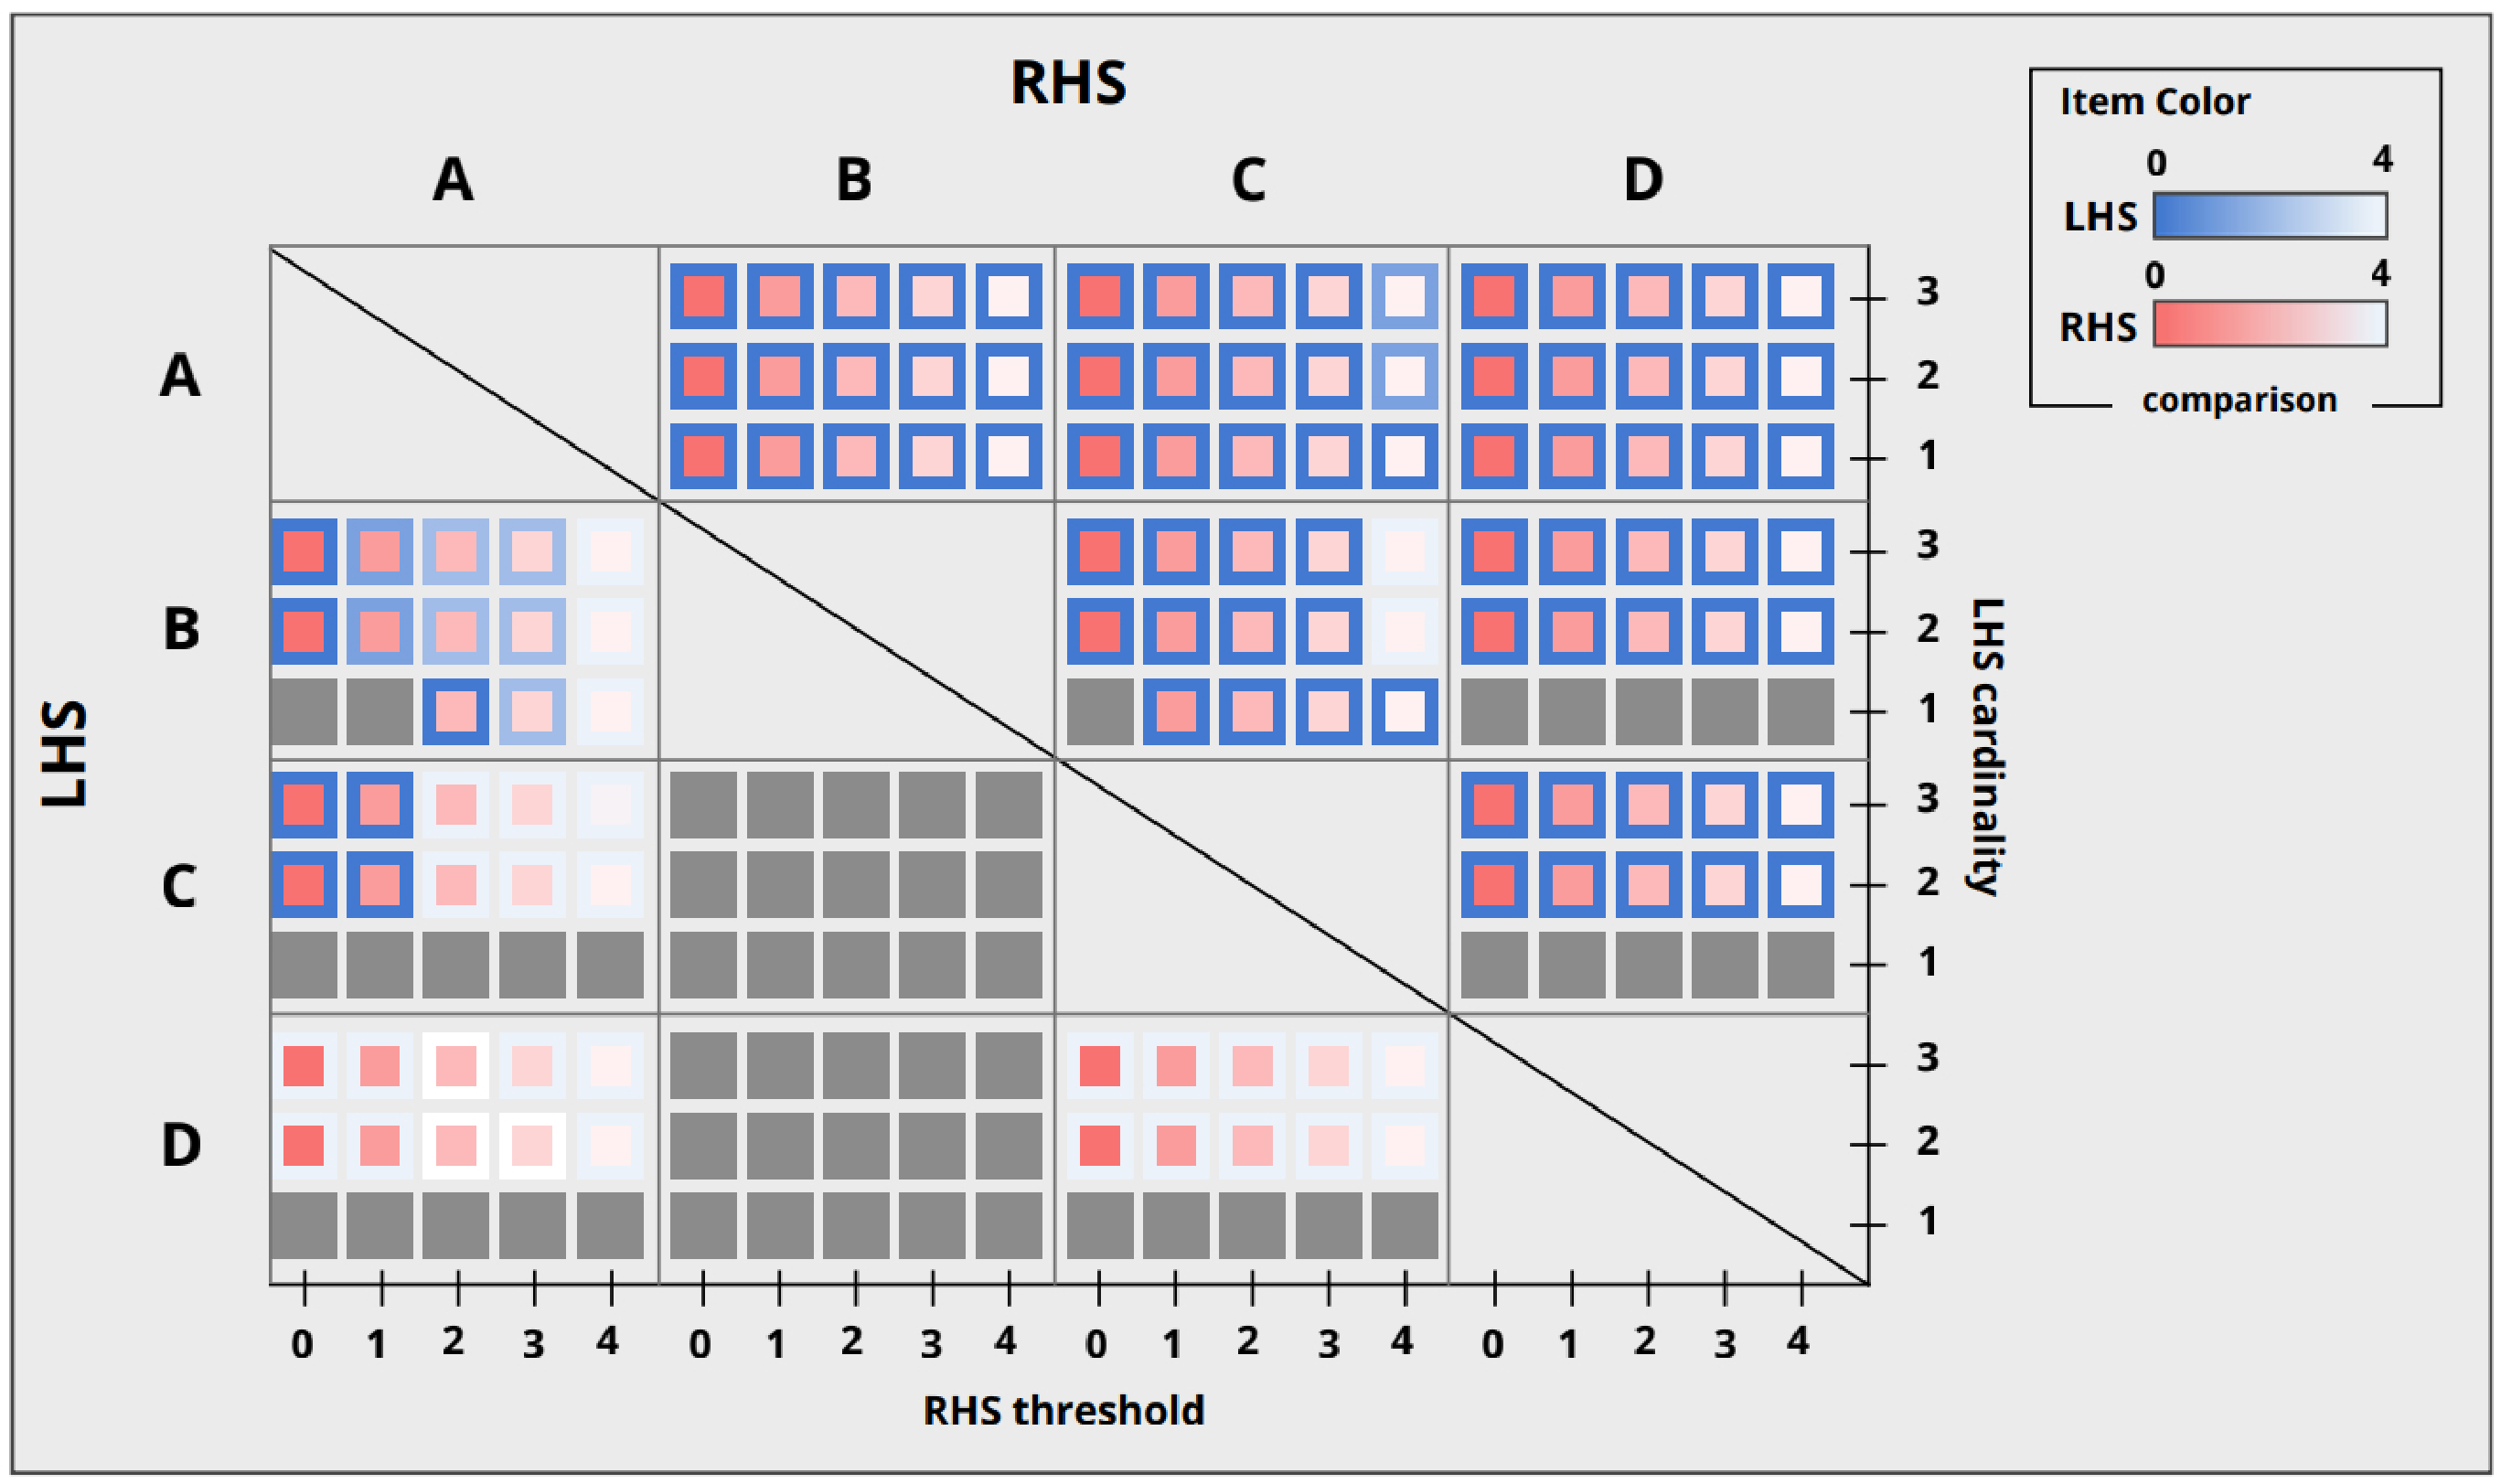
\includegraphics[width=\linewidth]{capitoli/figure/matrix_metaphore}
    \caption{Matrice colorata per una relazione con quattro attributi e soglie massime pari a 4.}
    \label{fig:colored_matrix}
\end{figure}
In questa sezione descriveremo una metafora per la visualizzazione di \acrshort{rfds} minimali \cite{mdvisualization}, scoperte dagli algoritmi di ricerca. La metafora che andremo a descrivere \`{e} una matrice colorata $n\times n$, come mostrato in Figura \ref{fig:colored_matrix}, dove $n$ rappresenta il numero di attributi. Questa prima metafora fornisce una panoramica sulle combinazioni di attributi su cui esiste una \acrshort{rfd} minimale, includendo la rappresentazione delle soglie di somiglianza corrispondenti basata su scale di gradienti di colore lineare. Come gi\`{a} accennato, le dimensioni della matrice rappresentano tutti gli attributi del dataset, utilizzando la stessa posizione per un dato attributo su entrambe le dimensioni. Le colonne di tale matrice, rappresentano i possibili attributi presenti sul lato destro, con le relative soglie associate. Le righe, invece, rappresentano le cardinalit\`{a} delle \acrshort{rfds} minimali includendo l'attributo di riga sul lato sinistro, con possibili soglie associate. Per esempio, consideriamo la sottomatrice $3\times5$ con le colonne associate all'attributo $A$ e le righe associate all'attributo $B$ nella Fig. \ref{fig:colored_matrix}. La riga in basso evidenzia se ci sono \acrshort{rfds} minimali con $B$ sul lato sinistro, la riga successiva evidenzia quelle che includono l'attributo $B$ con una cardinalit\`{a} del lato sinistra uguale a 2 (i.e., $BC$ o $BD$), ed infine, l'ultima riga evidenzia quelle che includono l'attributo $B$ con una cardinalit\`{a} del lato sinistro uguale a 3 (i.e., $BCD$). Le celle rappresentate in grigio indicano che non vi sono \acrshort{rfds} minimali con quelle caratteristiche, altrimenti sarebbero rappresentate con una sfumatura di rosso per lo sfondo ed il bordo con una sfumatura di blu. La sfumatura di rosso presente come sfondo delle celle rappresenta la soglia del lato destro, mentre la sfumatura di blu presente sul bordo delle celle rappresenta la soglia del lato sinistro, per cui colori pi\`{u} intensi rappresentano soglie pi\`{u} basse.\par
La matrice colorata, come descritta sopra, fornisce una panoramica delle correlazioni tra attributi mediante \acrlong{rfds}. Come esempio, il gruppo di colonne corrispondenti all'attributo $B$ nel lato destro mostrano che l'attributo \`{e} correlato solo all'attributo $A$, poich\'{e} le restanti sono tutte colorate di grigio. Allo stesso modo, il gruppo di colonne corrispondenti all'attributo $C$ sul lato destro rivelano che tale attributo ha pi\`{u} correlazioni con gli altri attributi, poich\'{e} ha poche celle colorate di grigio. Inoltre, guardando le ultime tre righe, si pu\`{o} notare che l'attributo $D$ appare nel lato sinistro di alcune \acrlong{rfds} solo in combinazione con altri attributi. Tali dipendenze hanno soglie alte sul lato sinistro (i bordi delle celle hanno un colore meno intenso) e consentono di ottenere \acrlong{rfds} minimali con soglie basse nel lato destro. Infine, la sotto-matrice corrispondente all'attributo di riga $B$ ed all'attributo di colonna $A$ rivela che esiste un'alta variabilit\`{a} delle soglie nelle \acrlong{rfds} aventi $B$ nel lato sinistro ed $A$ nel lato destro, poich\'{e} l'intensit\`{a} dei colori dei bordi diminuisce all'aumentare della soglia del lato destro.
\phantomsection
\chapter{Dependensee}
\markboth{Dependensee}{}
\label{cap5:dependensee}
% [titolo ridotto se non ci dovesse stare] {titolo completo}
In questo capitolo verr\`{a} introdotto \textit{Dependensee}, lo strumento sviluppato per la visualizzazione di insiemi minimali di \acrfull{rfds} mediante l'implementazione della metafora descritta nel paragrafo \ref{section:visual_rep_metaphore}. Questo facilita la visualizzazione delle \acrfull{rfds} minimali e rappresenta diverse loro caratteristiche, facilitando l'utente nell'analisi visiva.

\section{Blabla} %\label{1sec:scopo}
Capitolo x.1
\phantomsection
\chapter{Valutazione Sperimentale}
\markboth{Valutazione Sperimentale}{}
\label{cap5:valutazione_sperimentale}
% [titolo ridotto se non ci dovesse stare]
\section{Valutazione della metafora}
La metafora di visualizzazione descritta precedentemente \`{e} stata valutata \cite{mdvisualization} in uno studio qualitativo sottoposto ad utenti esperti, ovvero studenti del dottorato di ricerca ed amministratori di database, poich\'{e} l'obiettivo era valutare i task di analisi esplorativa, per i quali gli studi qualitativi si sono dimostrati pi\`{u} adatti delle misure quantitative \cite{informationvisualization,strategies4evaluatinginfo}. In particolare, lo studio \`{e} stato svolto con sei utenti in una sessione di due ore, nella quale gli utenti hanno utilizzato la metafora proposta con tre dataset pubblici tratti dalla repository della UCI Machine Learning \cite{ucirepository}: Breast-cancer, Bridges e Echocardiogram. Le statistiche delle caratteristiche dei dataset considerati ed il numero di \acrshort{rfds} trovate sono riportate nella Tabella \ref{table:1},
% -- Tabella dei risultati
\begin{table}[h!]
\centering
%\refstepcounter{table}
\begin{tabular}{|l|rrrr|r|} 
\hline
\multicolumn{1}{|c|}{\multirow{2}{*}{\textbf{Dataset}}} & \multicolumn{4}{c|}{\textbf{Statistiche}}                                                                                              & \multicolumn{1}{c|}{\multirow{2}{*}{\textbf{\#RFD Totali}}}  \\
\multicolumn{1}{|c|}{}                         & \multicolumn{1}{l}{\textbf{\#Colonne}} & \multicolumn{1}{l}{\textbf{\#Righe}} & \multicolumn{1}{l}{\textbf{\#FD}} & \multicolumn{1}{l|}{\textbf{Dimensione (KB)}} & \multicolumn{1}{c|}{}                                \\ 
\hline
Breast-cancer                                  & 11                            & 699                         & 46                       & 20                                   & 814                                                  \\
Bridges                                        & 13                            & 107                         & 142                      & 6                                    & 6960                                                 \\
Echocardiogram                                 & 13                            & 132                         & 538                      & 6                                    & 2396                                                 \\
\hline
\end{tabular}
\caption{Statistiche e risultati delle RFD scoperte sui dataset considerati.}
\label{table:1}
\end{table}
% -- Fine Tabella
mentre la metafora di visualizzazione applicata al dataset Echocardiogram \`{e} mostrata in Figura \ref{fig:colored_matrix_echo}.
% -- Metafora per le RFDs scovate in Echocardiogram
\begin{figure}[ht]
    \centering
    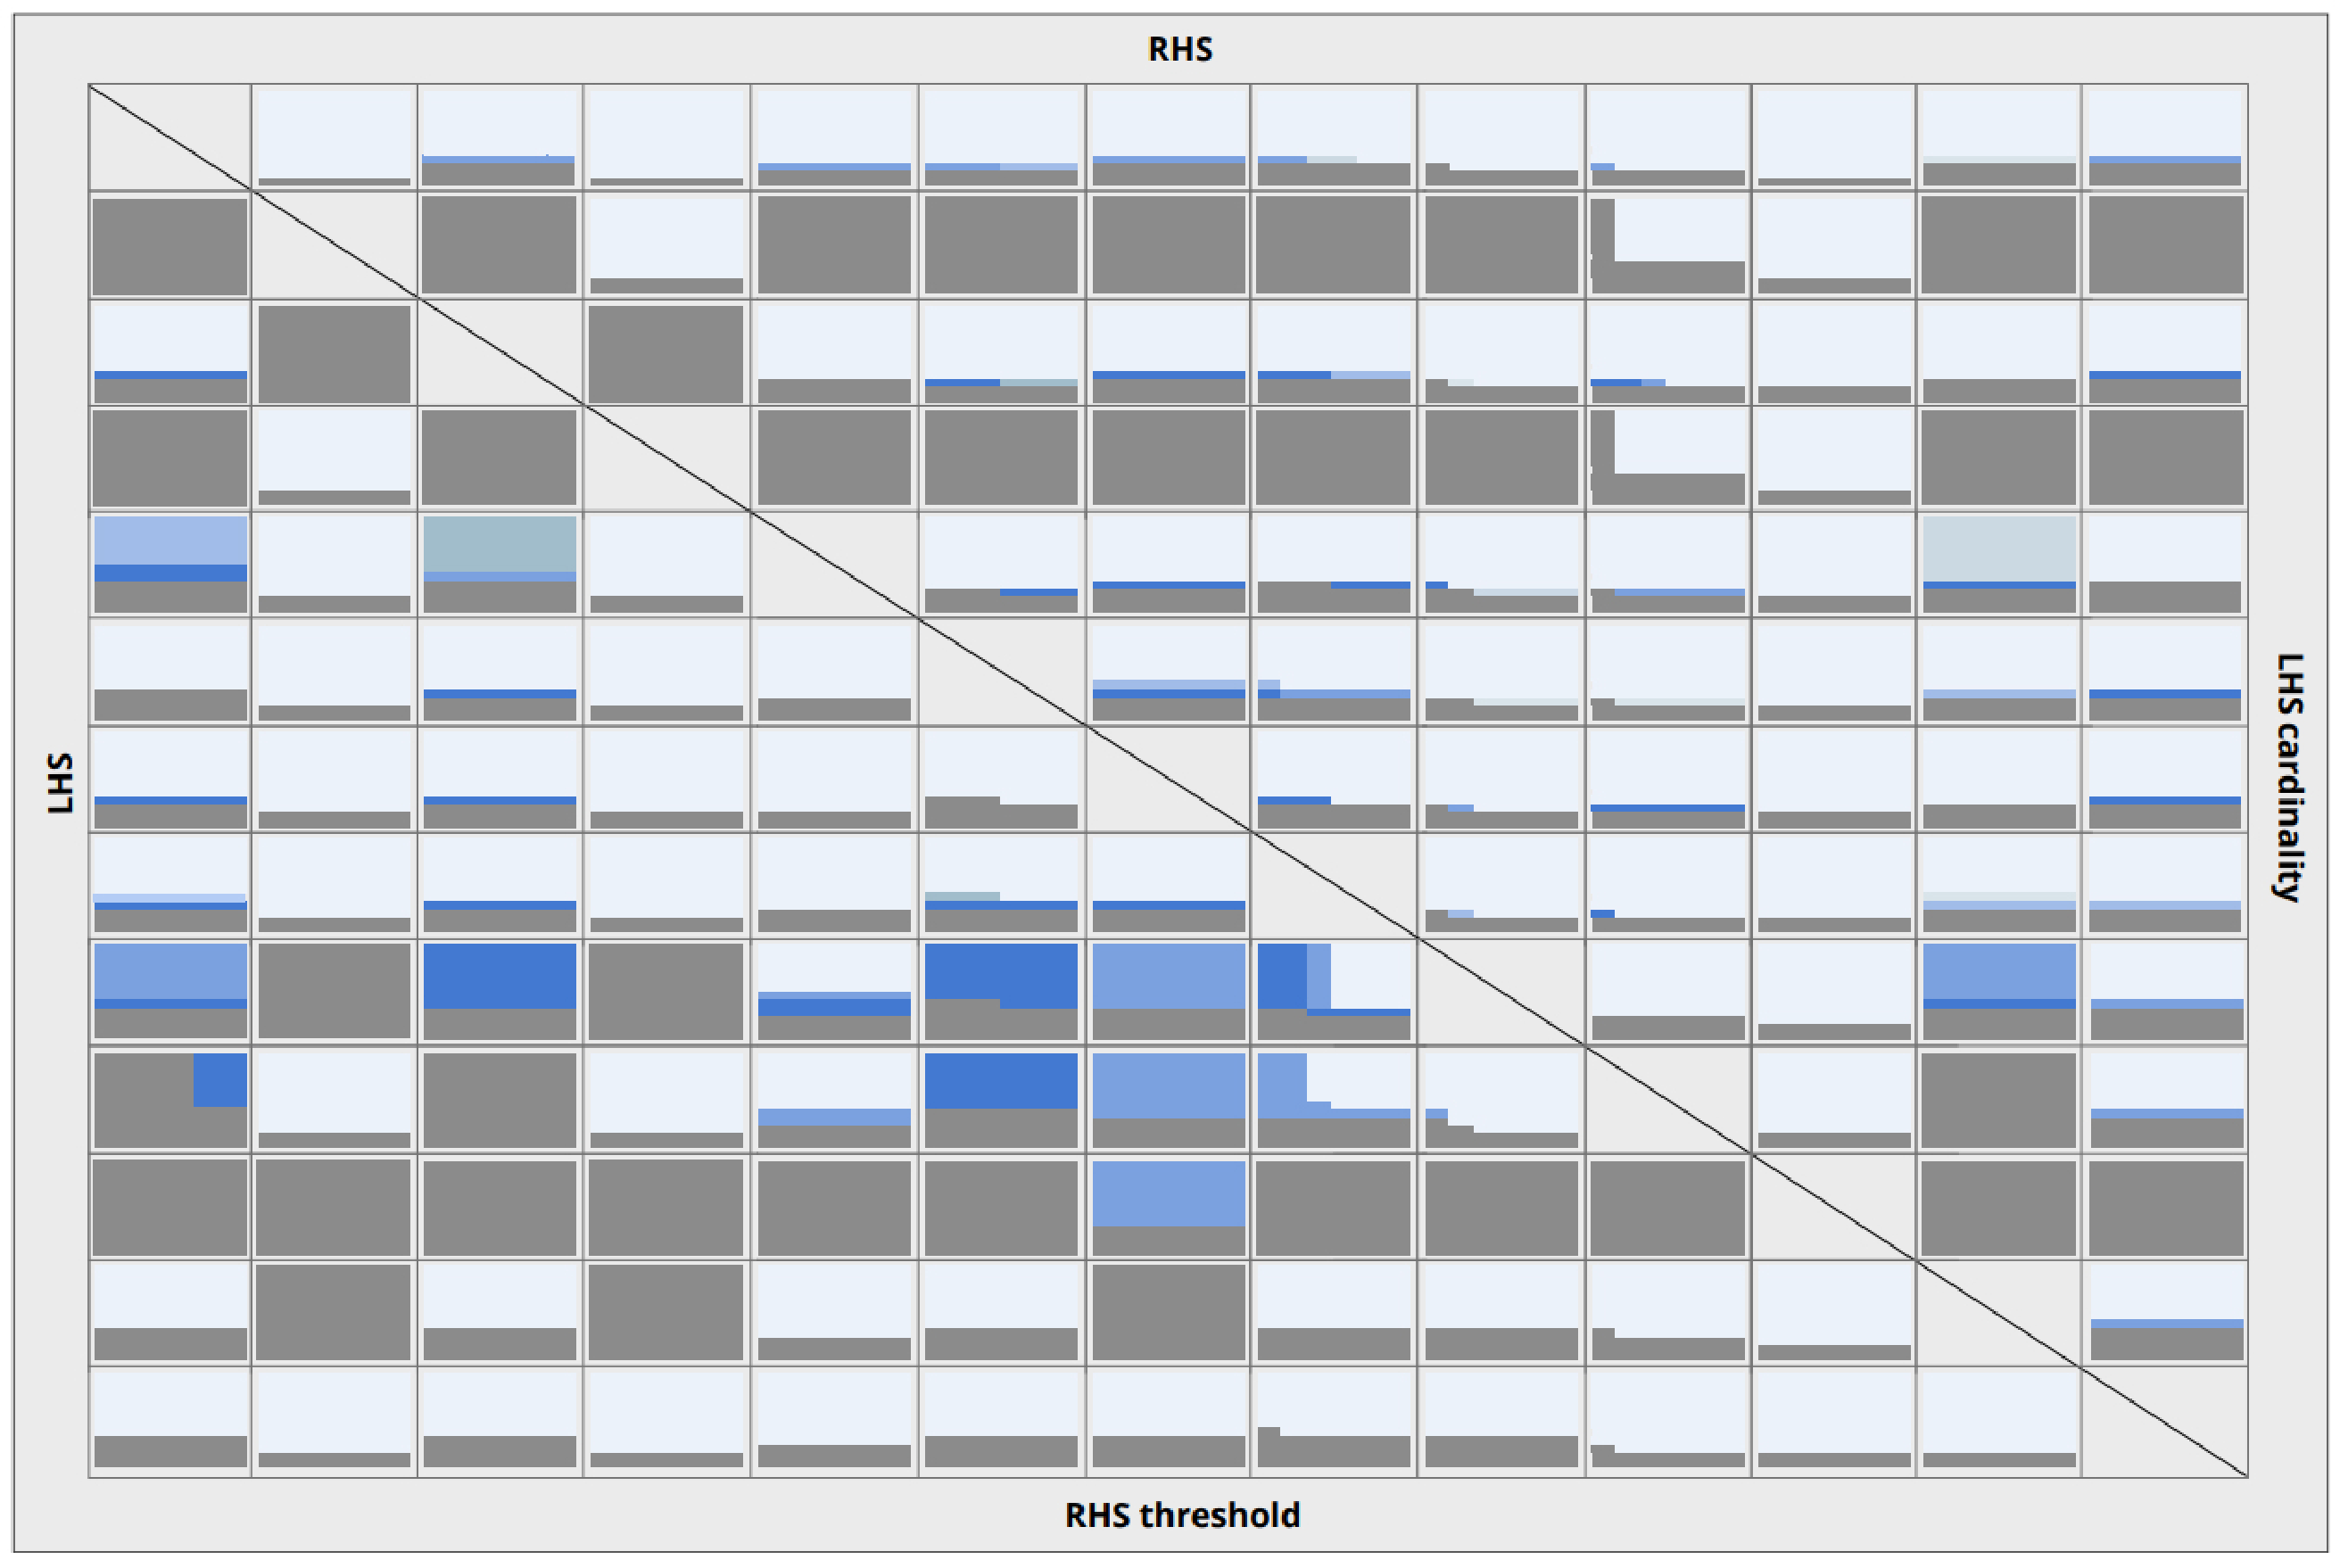
\includegraphics[width=\linewidth]{capitoli/figure/echo_metaphore}
    \caption{Matrice colorata per le \acrshort{rfds} estratte dal dataset Echocardiogram.}
    \label{fig:colored_matrix_echo}
\end{figure}
% -- Fine metafora
Al termine della sessione di valutazione, questi erano i feedback degli utenti in merito ai vantaggi delle metafore di visualizzazione proposte:
\begin{itemize}
    \item \textit{Coinvolgimento degli attributi nelle \acrshort{rfds}}: oltre alla frequenza con cui un attributo si presenta nelle \acrshort{rfds}, la matrice colorata ha fornito informazioni sulla loro frequenza di occorrenza sul lato sinistro o sul lato destro, affermando se un attributo \`{e} pi\`{u} implicato da un altro attributo oppure implica altri attributi;
    \item \textit{Cardinalit\`{a} del lato sinistro}: mentre la cardinalit\`{a} del lato destro delle \acrshort{rfds} trovate \`{e} sempre pari a $1$, quella del lato sinistro pu\`{o} variare tra $1$ ed il numero di attributi meno $1$. La matrice colorata fornisce un feedback immediato sulla cardinalit\`{a} del lato sinistro;
    \item \textit{Correlazione degli attributi}: per un dato attributo sul lato destro, tutti gli utenti hanno concordato sul fatto che la matrice colorata ha fornito un feedback immediato sulle correlazioni degli attributi, ovvero con quale frequenza due attributi si trovano su lati diversi della stessa \acrshort{rfd};
\end{itemize}
In sintesi, l'analisi della metafora proposta rivela che ha supportato con successo utenti esperti nell'analisi di enormi set di \acrshort{rfds} e le loro soglie associate. Soprattutto, ha fornito nuove panoramiche e astrazioni delle \acrshort{rfds} scoperte, riducendo considerevolmente lo sforzo necessario per analizzarle.

\section{Risultati}
Attraverso l'implementazione della metafora di visualizzazione esposta nel capitolo \ref{section:visual_rep_metaphore} all'interno di Dependensee, si \`{e} riusciti a rappresentare in modo immediato ed efficace un dataset di \acrlong{rfds} minimali. In questo modo \`{e} stato possibile effettuare un'analisi visiva quasi istantanea, grazie alle diverse caratteristiche messe in luce dalla rappresentazione grafica fornita dallo strumento. Infatti, questa rappresentazione raffigura le dipendenze minimali esistenti tra tutti gli attributi contenute nel dataset, mettendo in risalto la cardinalit\`{a} del lato sinistro e le soglie associate sia per il lato sinistro che per il lato destro.\par
% -- TAB DATASET --
\begin{table}[ht]
\centering
\begin{tabular}{|lrrr|} 
\hline
\multicolumn{4}{|c|}{\textbf{Statistiche}}                                                                                                \\
\textbf{Dataset} & \multicolumn{1}{c}{\textbf{\#Attributi}} & \multicolumn{1}{c}{\textbf{\#Tuple}} & \multicolumn{1}{l|}{\textbf{\#RFD}}  \\ 
\hline
Echocardiogram   & 13                                       & 132                                    & 2396                                 \\
Citiseer   & 7                                        & 2000                                    & 107                                  \\
Car\_data        & 7                                        & 1729                                    & 8                                    \\
Restaurant       & 6                                        & 864                                    & 1961                                 \\
Foodstamp        & 5                                        & 150                                    & 9                                    \\
expIDEAS         & 3                                        & 7                                    & 12                                   \\
\hline
\end{tabular}
\caption{Statistiche dei dataset analizzati con Dependensee.}
\label{table:datasets_analyzed_stats}
\end{table}
% -- END TAB DATASET --
La valutazione \`{e} avvenuta attraverso l'analisi dei dataset elencati nella Tabella \ref{table:datasets_analyzed_stats}, i quali presentano caratteristiche differenti, come il numero di attributi, il numero di tuple ed il numero di \acrshort{rfds} individuate.
\begin{figure}[ht]
    \centering
    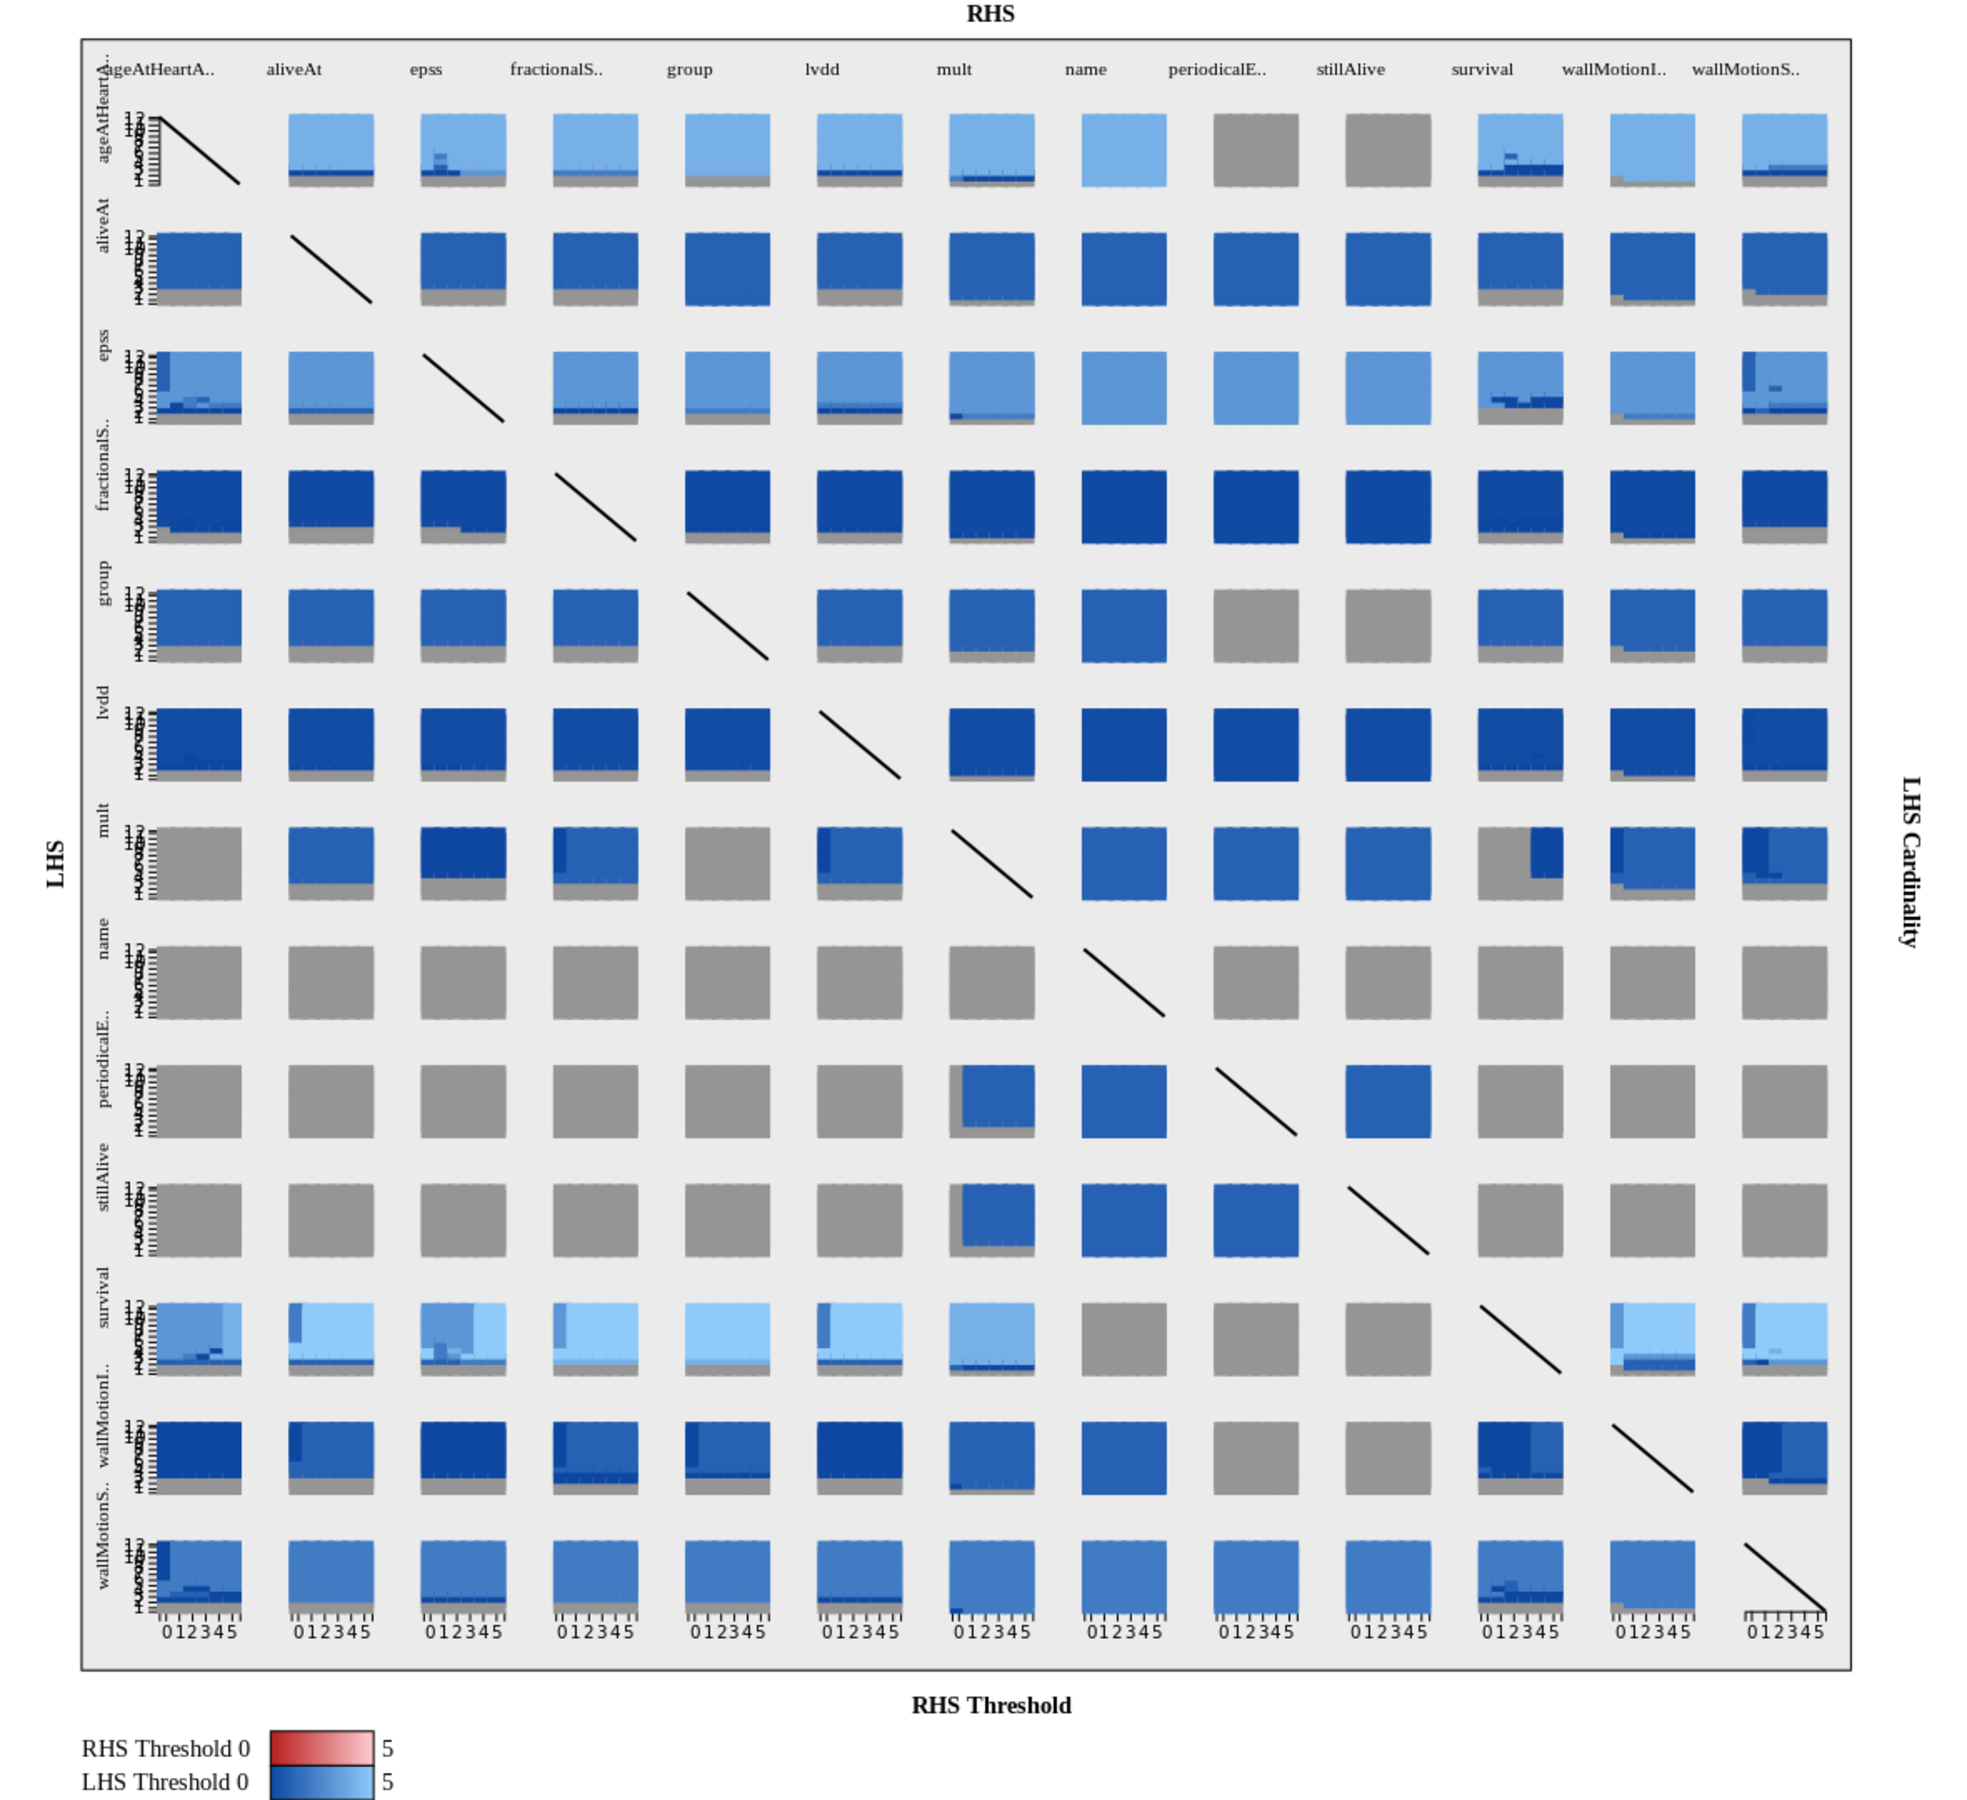
\includegraphics[width=\linewidth]{capitoli/figure/echocardiogram}
    \caption{Rappresentazione ottenuta in output da Dependensee del dataset Echocardiogram.}
    \label{fig:echocardiogram_result}
\end{figure}
La Figura \ref{fig:echocardiogram_result} mostra la grafica ottenuta analizzando il dataset \textit{Echocardiogram} con Dependensee. Da un primo sguardo si pu\`{o} notare come questa faciliti effettivamente l'analisi visuale per l'utente. Analizzando il dataset attraverso tale rappresentazione possiamo notare, mediante la diagonale nulla, come le \acrlong{rfds} banali non vengano rappresentate. In questo caso, data la grande mole di attributi, il grafico risultante enfatizza la soglia del lato sinistro piuttosto che quella del lato destro, essendo quest'ultima fissata. Inoltre, le label di alcuni attributi vengono troncate in quanto troppo lunghe, per evitare che queste si sovrappongano alle altre label. Il dataset \`{e} stato analizzato con una soglia massima data in input pari a $5$ e la gran parte delle \acrlong{rfds} minimali hanno la soglia minima o un valore vicino al minimo sul lato sinistro, poche con una soglia di valore massimo. Dalla Figura \ref{fig:echocardiogram_result} possiamo notare che non esistono \acrlong{rfds} minimali con l'attributo \texttt{name} sul lato sinistro con soglia tra $0$ e $5$, in quanto tutta la riga \`{e} di color grigio. Se osserviamo, invece, la prima riga e la seconda colonna, possiamo notare l'esistenza di \acrlong{rfds} minimali di cardinalit\`{a} $3$ con soglia minima e le \acrlong{rfds} minimali con cardinalit\`{a} maggiore sono tutte con soglia massima. Se consideriamo la riga con l'attributo \texttt{ageAtHearthAttack} sul lato sinistro e la colonna con l'attributo \texttt{name} sul lato destro, ovvero prima riga ed ottava colonna, possiamo notare che tutte le \acrlong{rfds} minimali sono con soglia massima pari a $5$, difatti tutta la sotto-matrice presenta il colore pi\`{u} chiaro. Da un'analisi generale, invece, si pu\`{o} notare che la gran parte delle \acrlong{rfds} minimali sono con soglia minima pari a $0$, molte con soglia di valore medio tra $1$ e $4$, poche con soglia pari al valore massimo $5$.\par
\begin{figure}[ht]
    \centering
    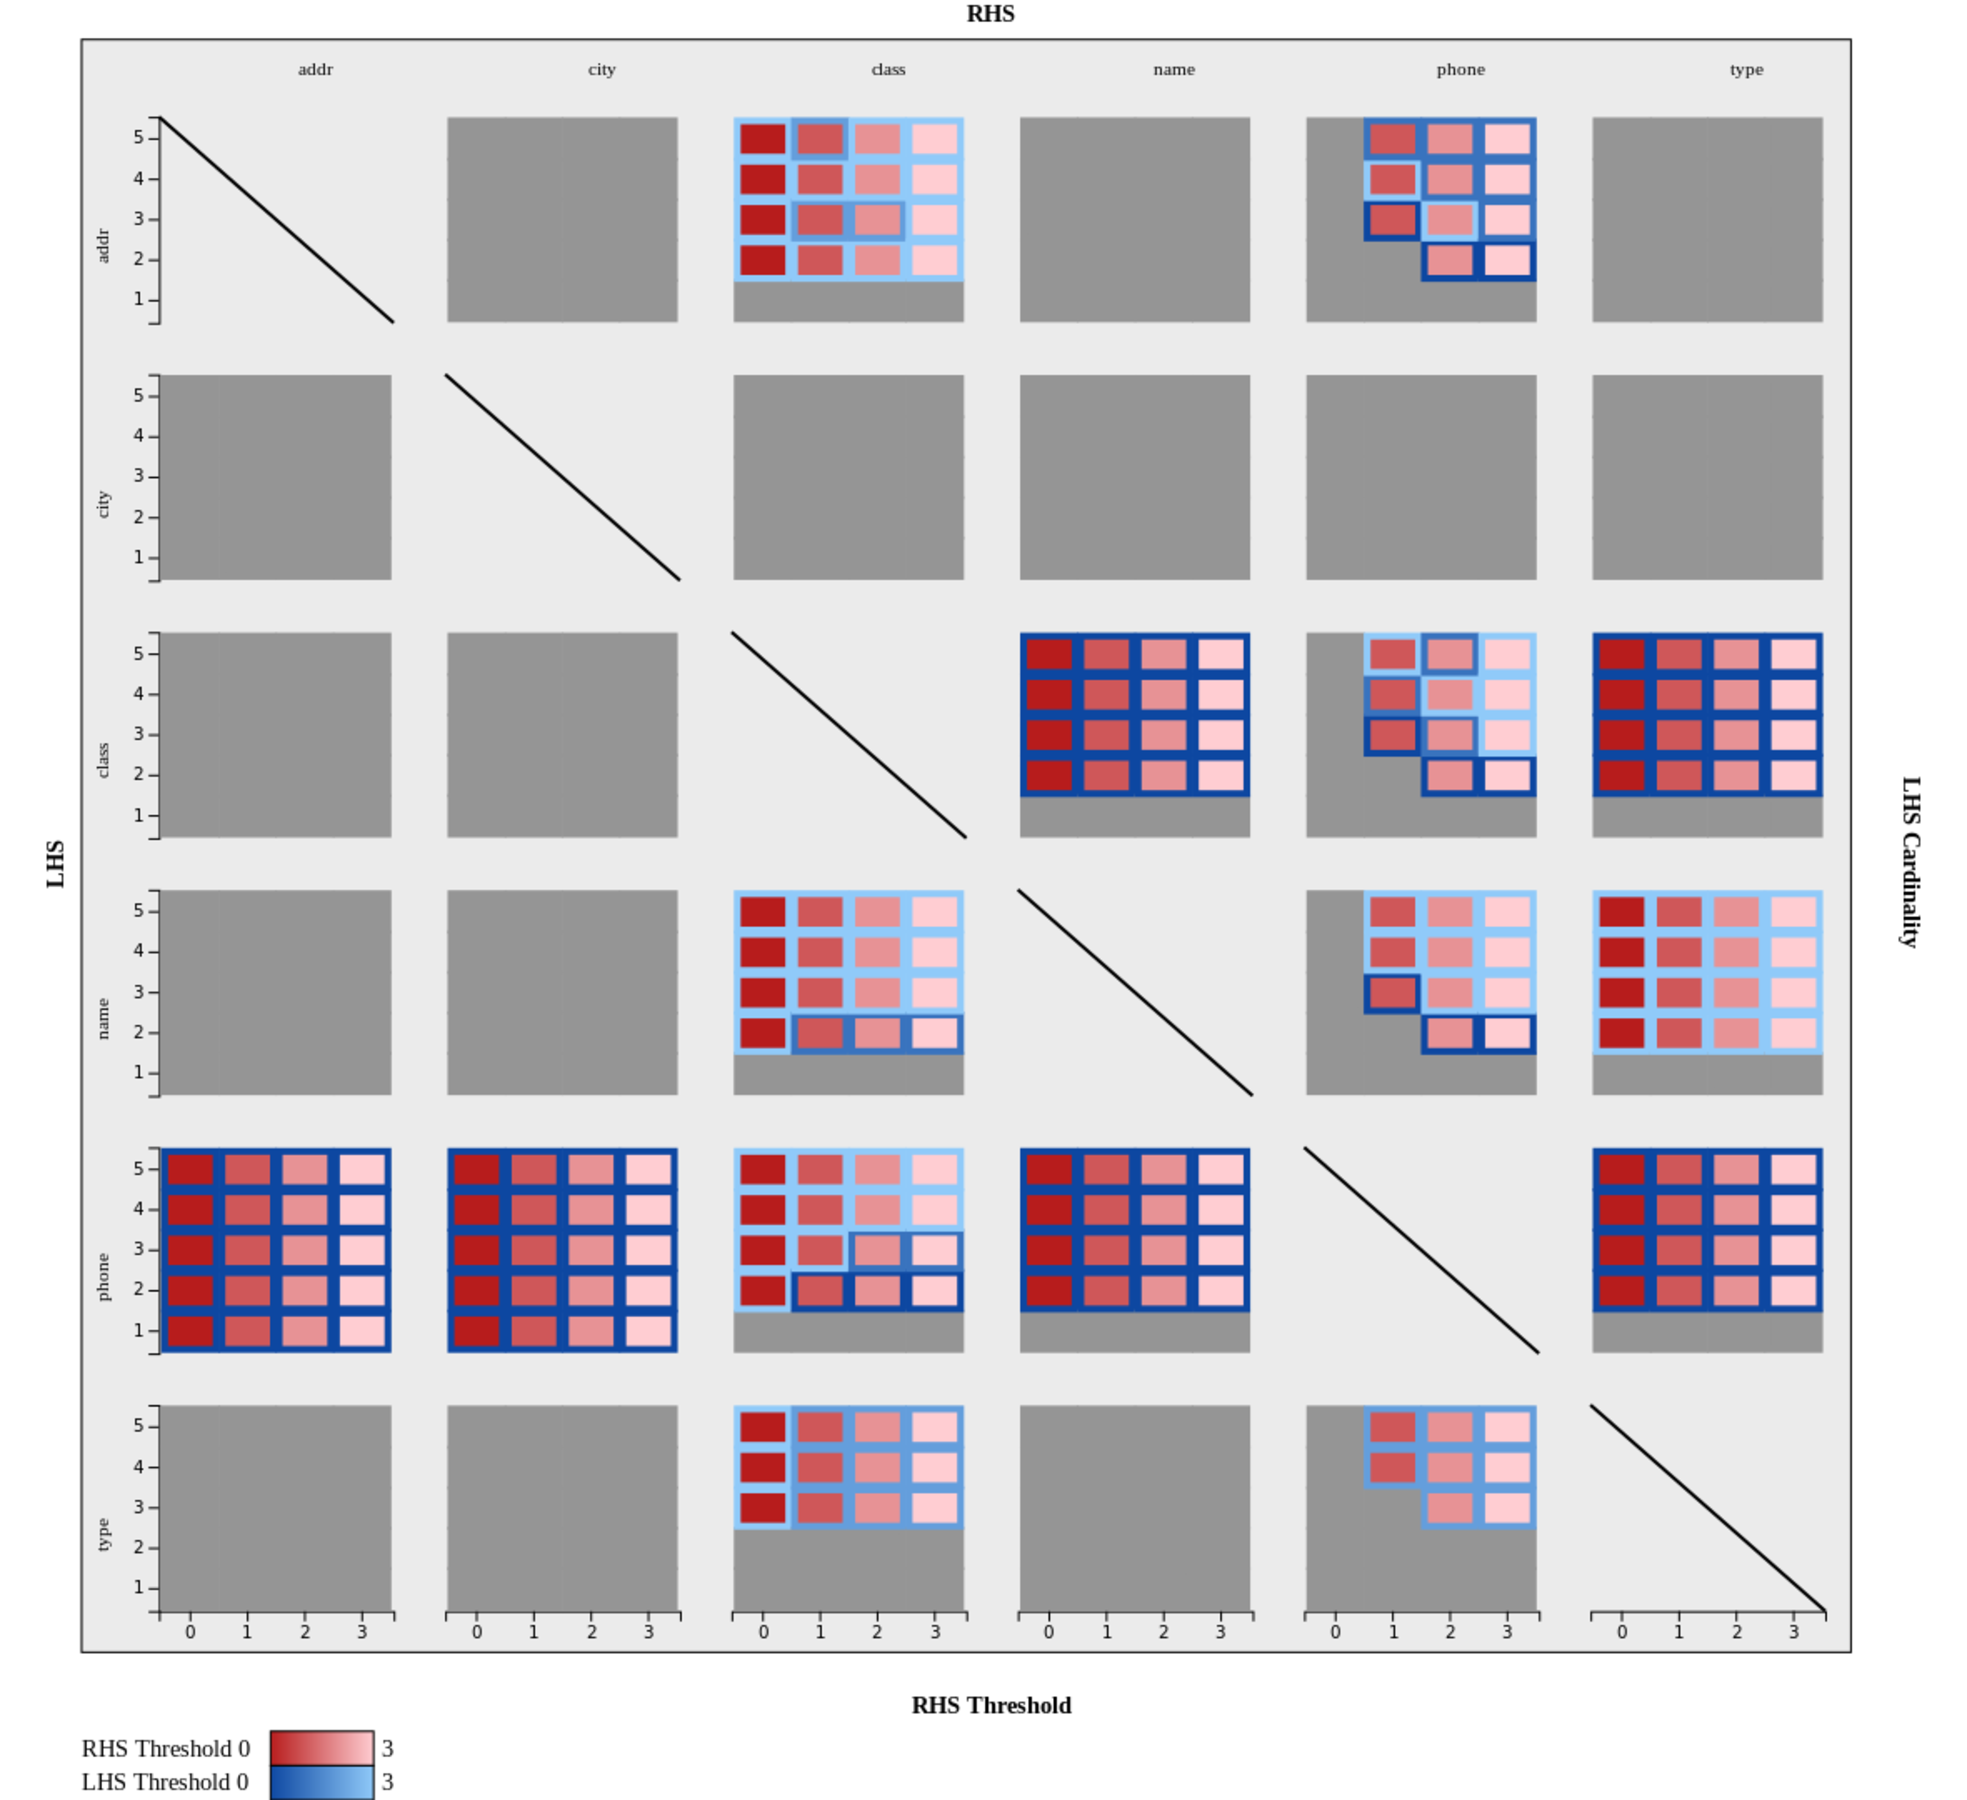
\includegraphics[width=\linewidth]{capitoli/figure/restaurant}
    \caption{Rappresentazione ottenuta in output da Dependensee del dataset Restaurant.}
    \label{fig:restaurant_result}
\end{figure}
Per quanto concerne l'analisi del dataset \textit{Restaurant}, la Figura \ref{fig:restaurant_result} mostra la rappresentazione grafica ottenuta mediante l'utilizzo di Dependensee. Da un'analisi generale si pu\`{o} affermare che le \acrlong{rfds} minimimali esistenti sono distribuite e non coprono tutti gli attributi del dataset. Infatti, la seconda riga \`{e} totalmente grigia, segno che non esiste alcuna \acrlong{rfds} minimale con l'attributo \texttt{city} sul lato sinistro. Continuando, vi sono molte altre sotto-matrici grigie che indicano l'assenza di \acrlong{rfds} minimali. Ci\`{o} non \`{e} uguale per tutte le sotto-matrici del grafico. Se consideriamo la riga relativa all'attributo \texttt{phone}, questa presenta \acrlong{rfds} minimali per tutti gli attributi. Le \acrlong{rfds} minimali con l'attributo \texttt{phone} sul lato sinistro, in relazione con gli attributi \texttt{addr}, \texttt{city}, \texttt{name} e \texttt{type} sul lato destro, sono tutte soglia minima sul lato sinistro. Mentre, la maggior parte di quelle in relazione con l'attributo \texttt{class} sul lato destro hanno soglia massima, alcune hanno soglia minima o quasi. Se, invece, consideriamo la terza colonna relativa all'attributo \texttt{class} sul lato destro, possiamo notare che quasi tutte le \acrlong{rfds} minimali hanno soglia massima o molto vicina a questa sul lato sinistro. Invece, la colonna relativa all'attributo \texttt{addr} sul lato destro, presenta solo \acrlong{rfds} minimali con soglia minima sul lato sinistro in relazione con l'attributo \texttt{phone}. Considerando, invece, la colonna relativa all'attributo \texttt{name} sul lato destro, presenta solo \acrlong{rfds} minimali con soglia minima sul lato sinistro relative agli attributi \texttt{class} e \texttt{phone}. Invece, l'ultima colonna relativa all'attributo \texttt{type} presenta \acrlong{rfds} minimali solo con gli attributi \texttt{class}, \texttt{name} e \texttt{phone}. Quelle relative agli attributi \texttt{class} e \texttt{phone} sul lato destro sono tutte con soglia minima, mentre quelle relative all'attributo \texttt{name} sono tutte con soglia massima.\par
\begin{figure}[ht]
    \centering
    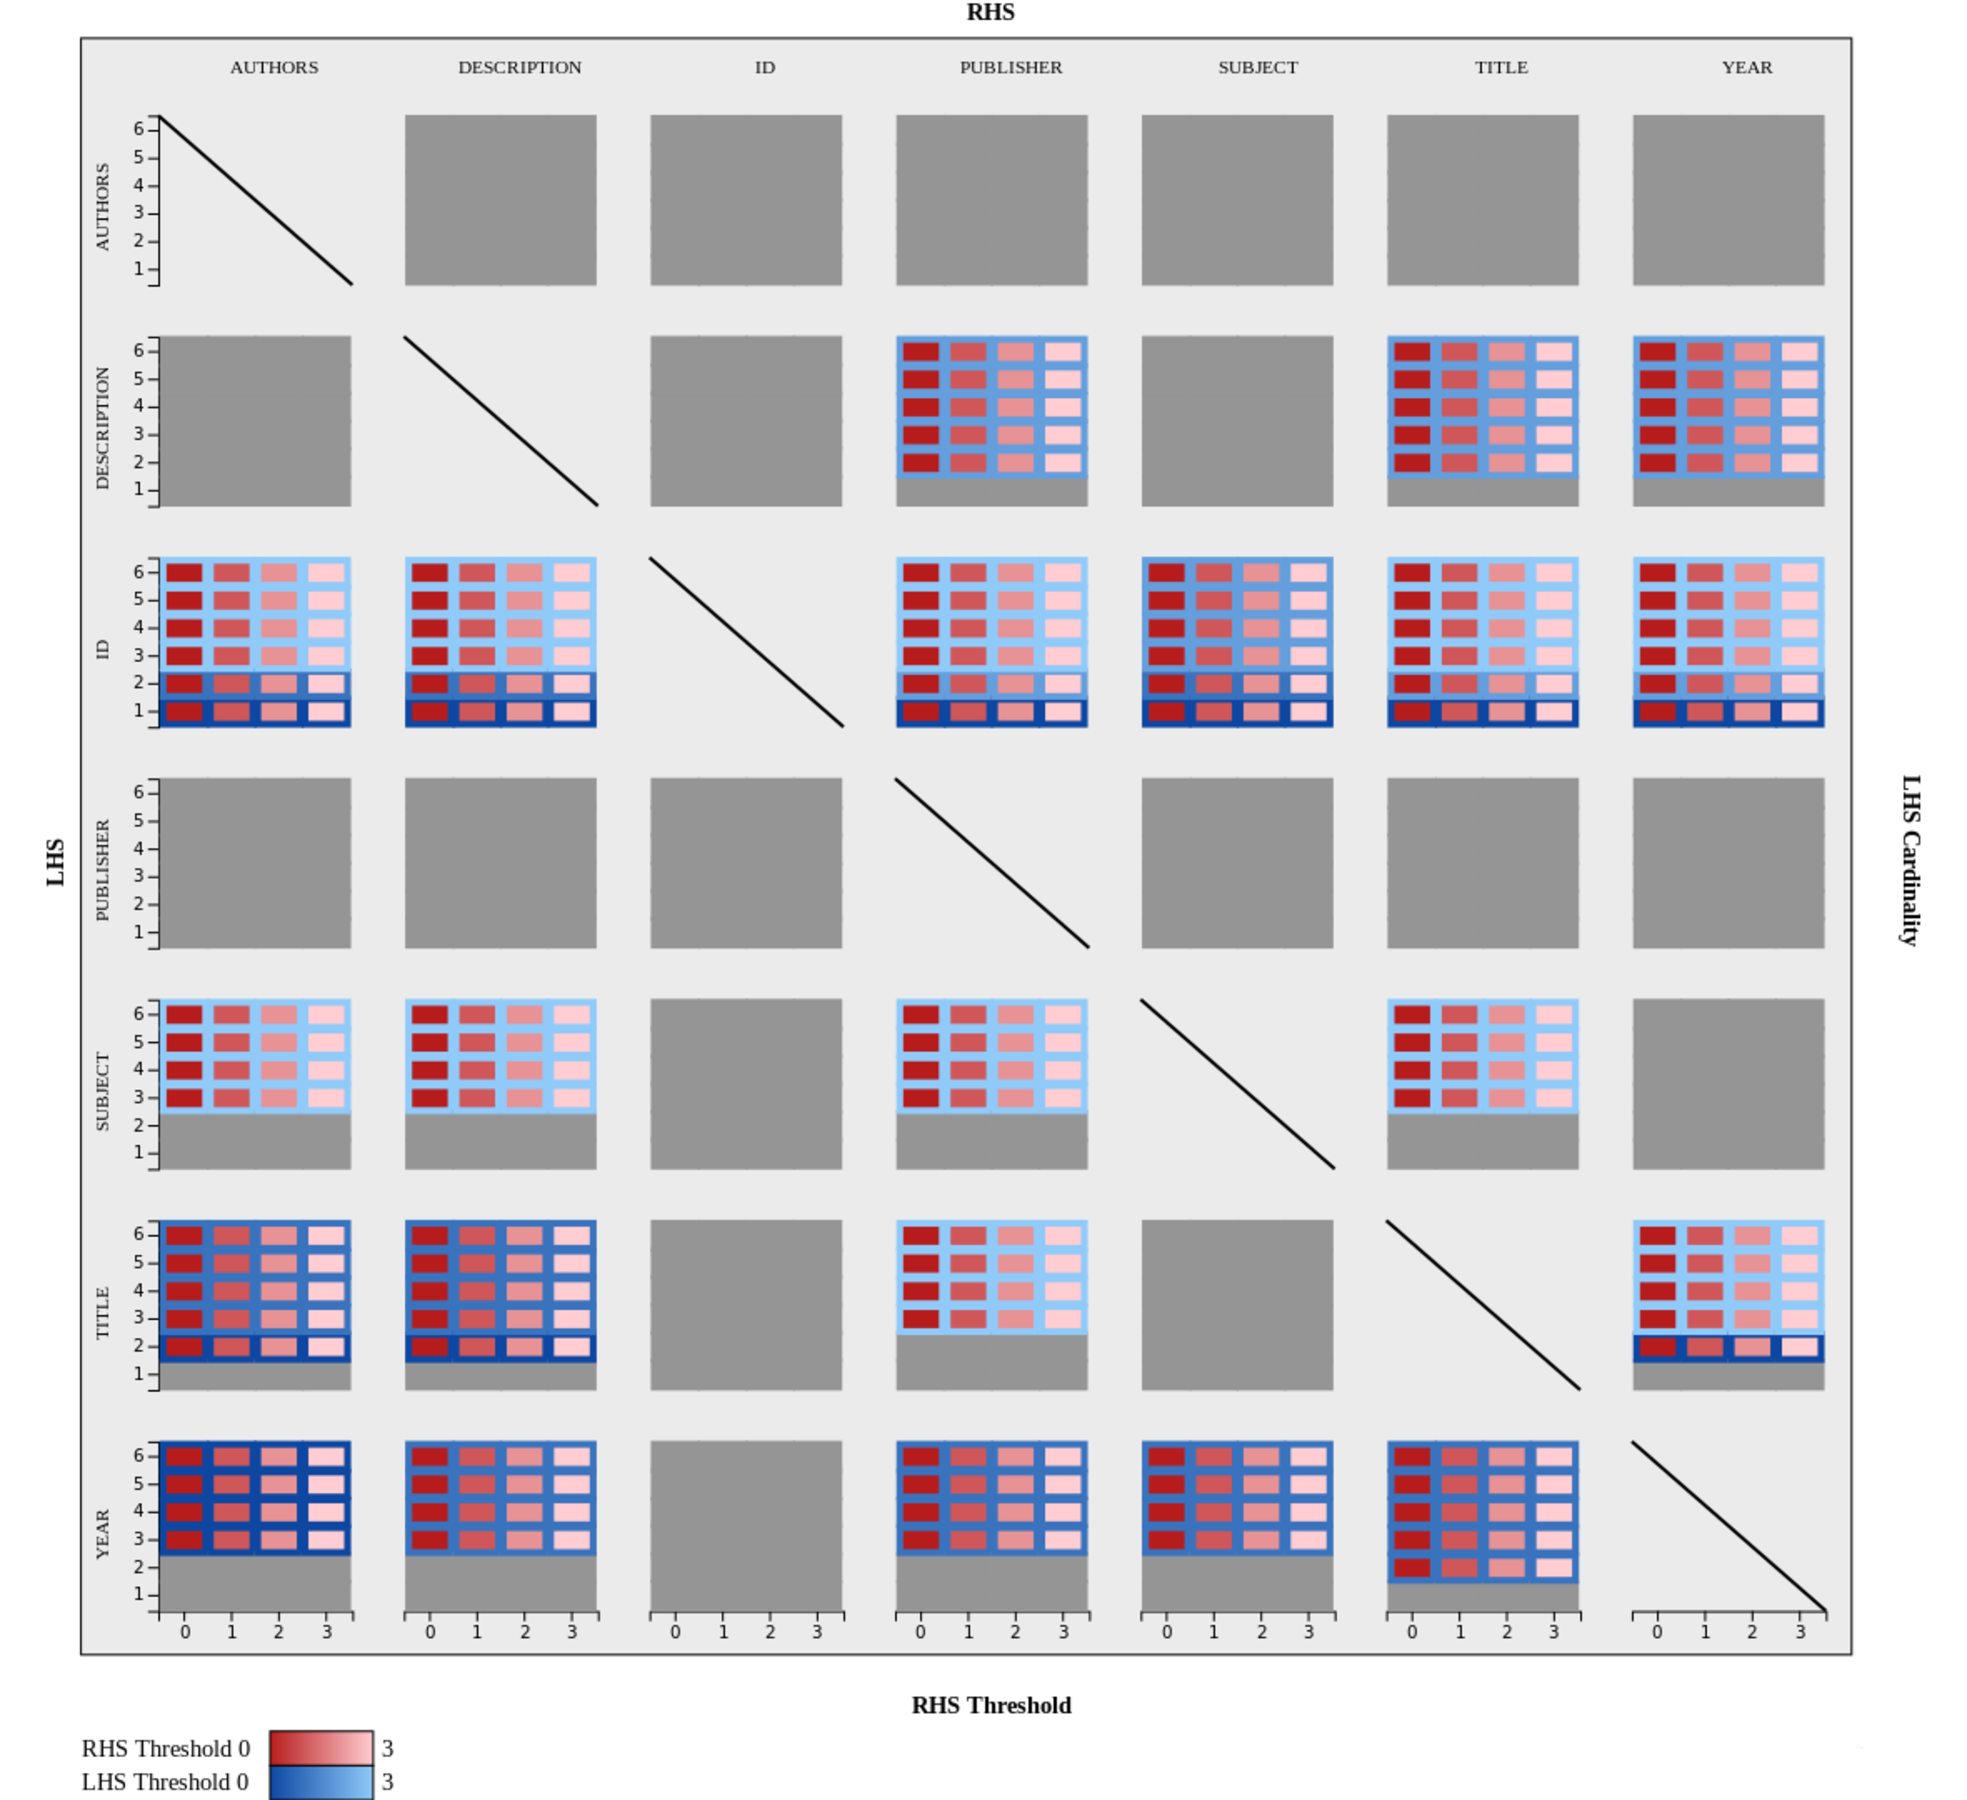
\includegraphics[width=\linewidth]{capitoli/figure/citiseer_2000_result}
    \caption{Rappresentazione ottenuta in output da Dependensee del dataset Citiseer.}
    \label{fig:citiseer_2000_result}
\end{figure}
La Figura \ref{fig:citiseer_2000_result} mostra la rappresentazione grafica ottenuta analizzando il dataset \textit{Citiseer} con Dependensee. Visto il basso numero di attributi, il grafico mostrer\`{a} anche il colore di riempimento relativo alla soglia del lato destro. Se prendiamo in considerazione la prima riga, possiamo notare come non esistano \acrlong{rfds} minimali con l'attributo \texttt{AUTHORS} sul lato sinistro e con almeno un attributo diverso sul lato destro, infatti tutta la riga \`{e} grigia. Analogamente con la terza riga, relativa all'attributo \texttt{PUBLISHER}. Mentre, con la colonna relativa all'attributo \texttt{ID}, possiamo notare l'assenza di \acrlong{rfds} minimali con l'attributo relativo sul lato destro. Se analizziamo la sotto-matrice relativa all'attributo riga \texttt{TITLE} ed all'attributo colonna \texttt{AUTHORS}, possiamo notare l'assenza di \acrlong{rfds} con cardinalit\`{a} pari a $1$ e l'esistenza di \acrlong{rfds} minimali con soglia pari a $0$ sul lato sinistro e cardinalit\`{a} pari a $2$, mentre per cardinalit\`{a} maggiori vi sono \acrlong{rfds} con soglia diverse da $0$ ma con valori vicini a questo.
Pi\`{u} in generale, la prima riga mostra l'esistenza di \acrlong{rfds} minimali con valore di soglia vicino al massimo inserito per l'analisi, ovvero $3$. La terza riga, invece, mostra la vasta presenza di \acrlong{rfds} minimali, molte con soglia pari al minimo o vicino a questo. La quinta riga, invece, mostra l'esistenza di \acrlong{rfds} minimali, tutte con valore di soglia minimo. L'ultima riga, invece, rappresenta le \acrshort{rfds} minimali, tutte con valore della soglia uguale al minino o vicino a questo.\par
\begin{figure}[H]
    \centering
    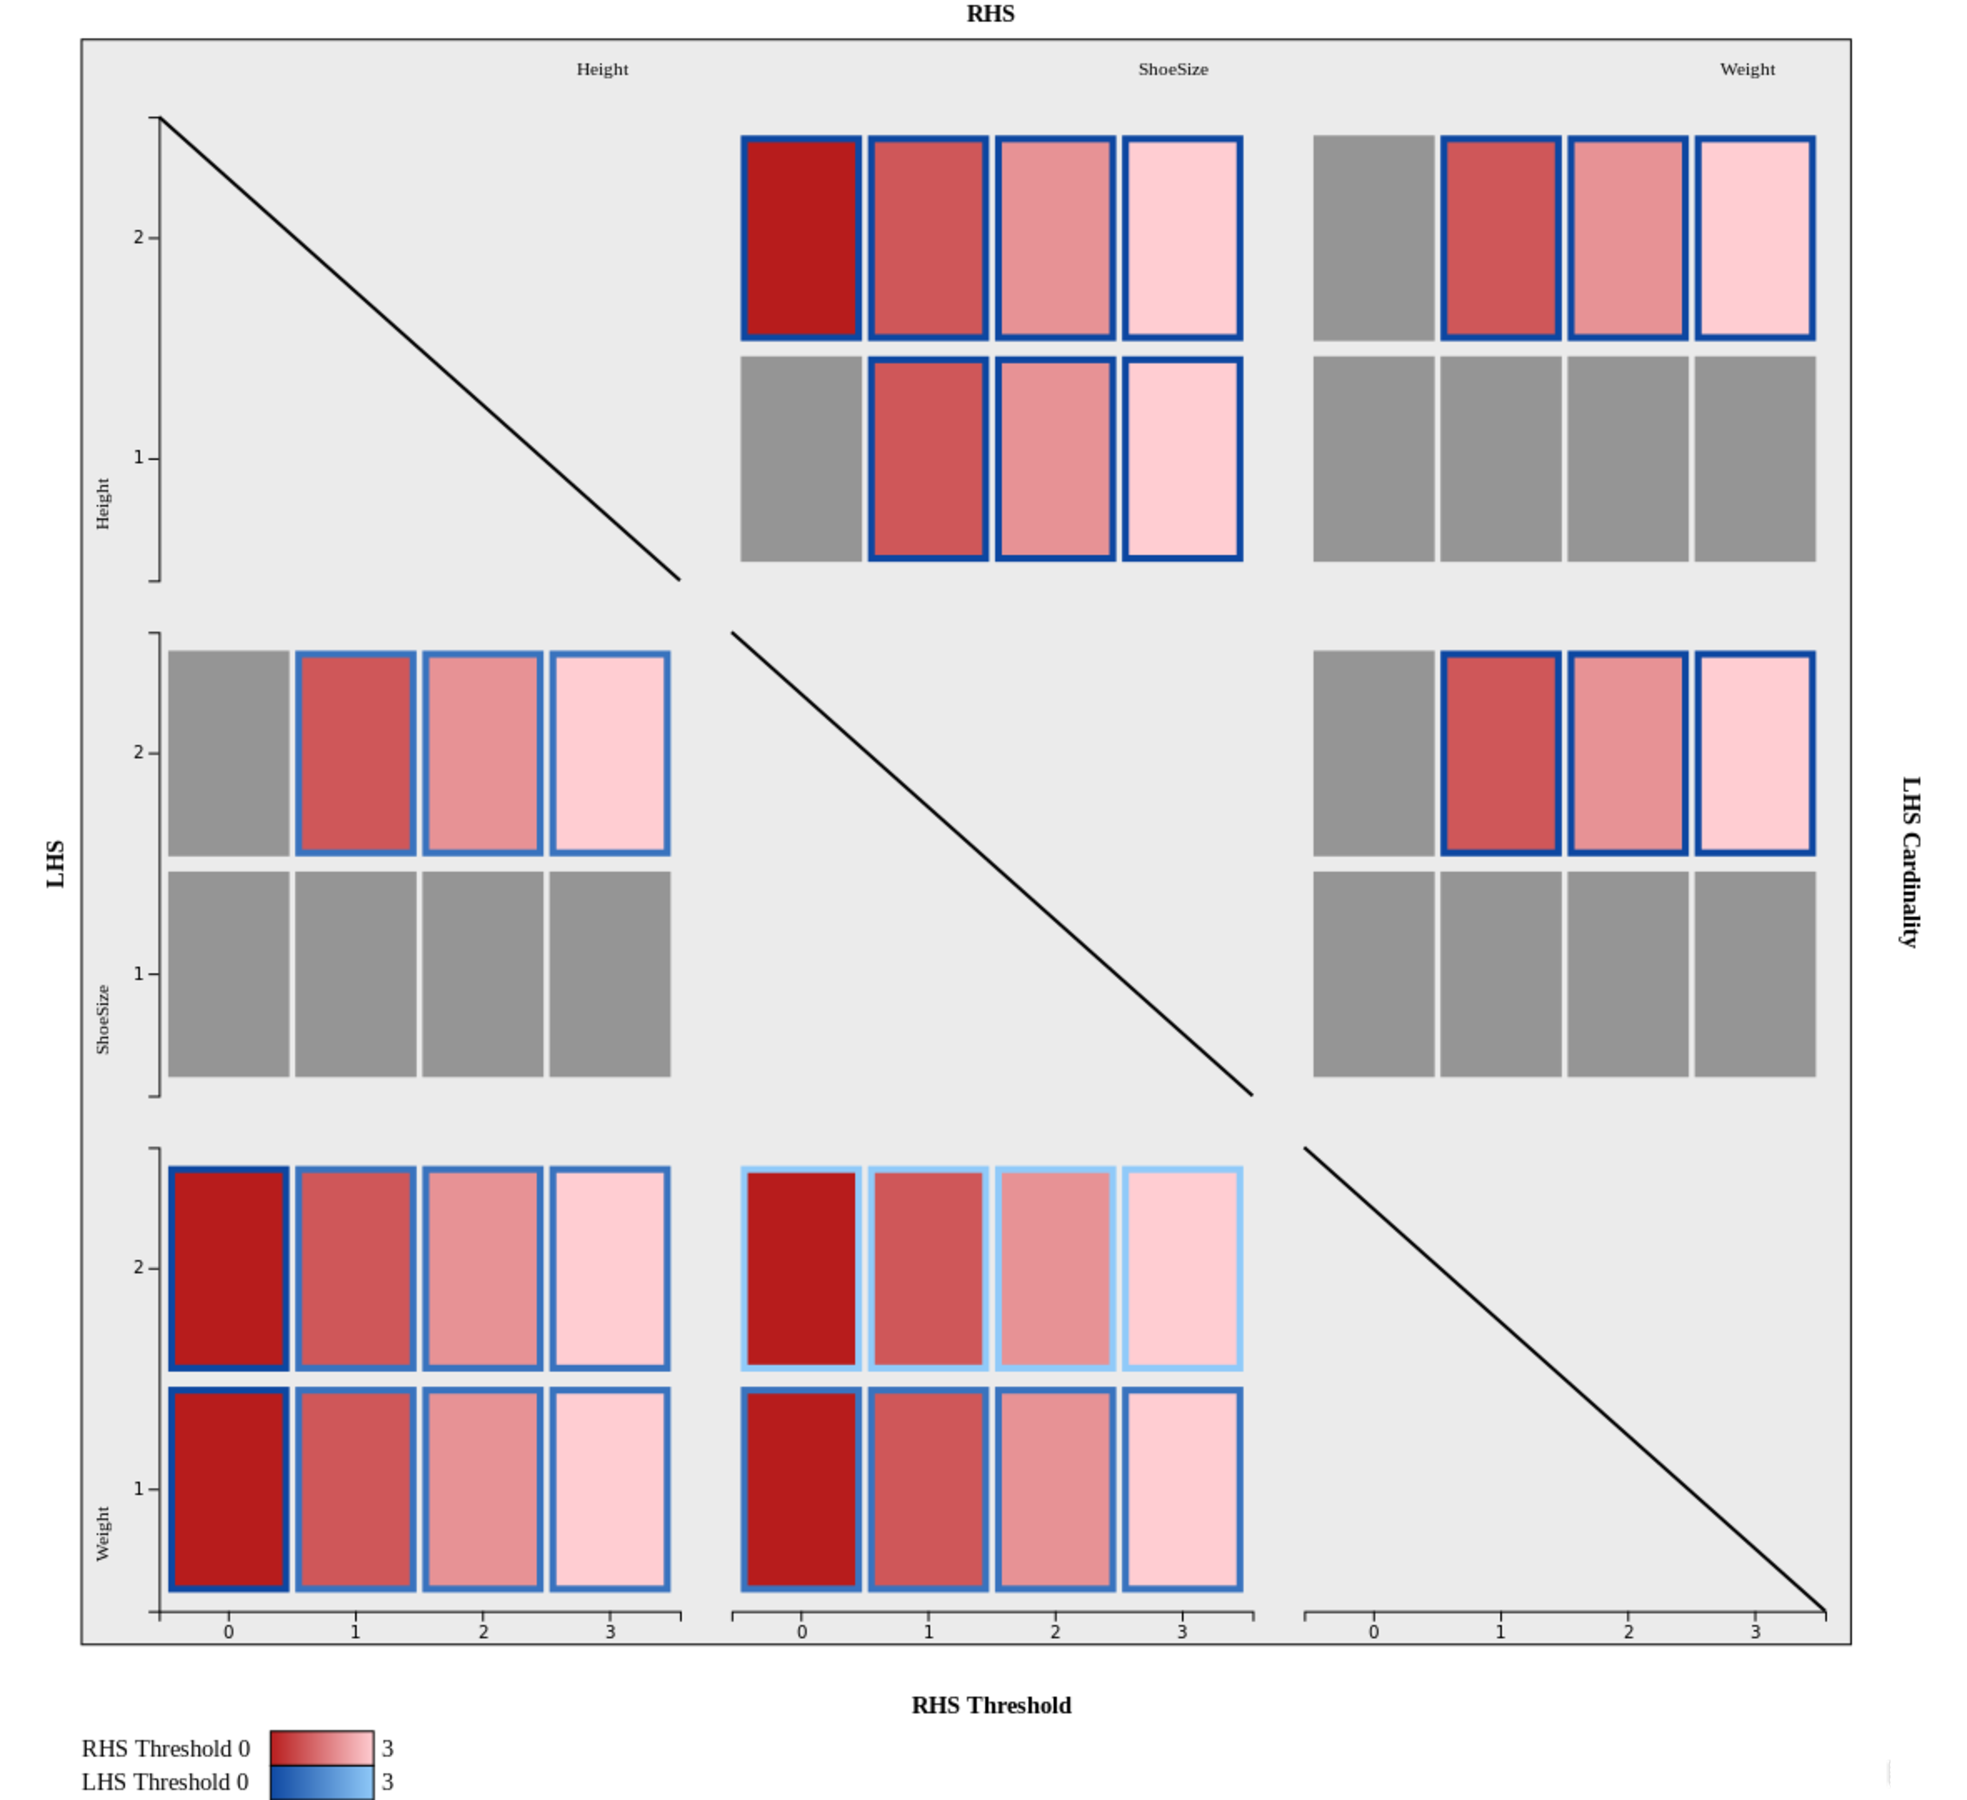
\includegraphics[width=\linewidth]{capitoli/figure/expIDEAS}
    \caption{Rappresentazione ottenuta in output da Dependensee del dataset expIDEAS.}
    \label{fig:expidea_result}
\end{figure}
La Figura \ref{fig:expidea_result} rappresenta il grafico ottenuto analizzando il dataset \textit{expIDEAS} mediante Dependensee. Il dataset contiene soltanto $3$ attributi e $12$ \acrlong{rfds} minimali. Dalla rappresentazione si pu\`{o} notare che le \acrlong{rfds} minimali sono ben distribuite. Con la prima riga possiamo notare che l'attributo \texttt{Height} sul lato sinistro figura in \acrlong{rfds} minimali con soglia minima. Anche con l'ultima colonna possiamo notare che l'attributo \texttt{Weight} sul lato destro figura in \acrlong{rfds} minimali con soglia minima. Invece, con l'ultima riga si pu\`{o} notare che l'attributo \texttt{Weight} sul lato sinistro figura in \acrlong{rfds} minimali, molte delle quali con soglia vicino o pari al massimo e poche con soglia pari al minimo.\par
\begin{figure}[ht]
    \centering
    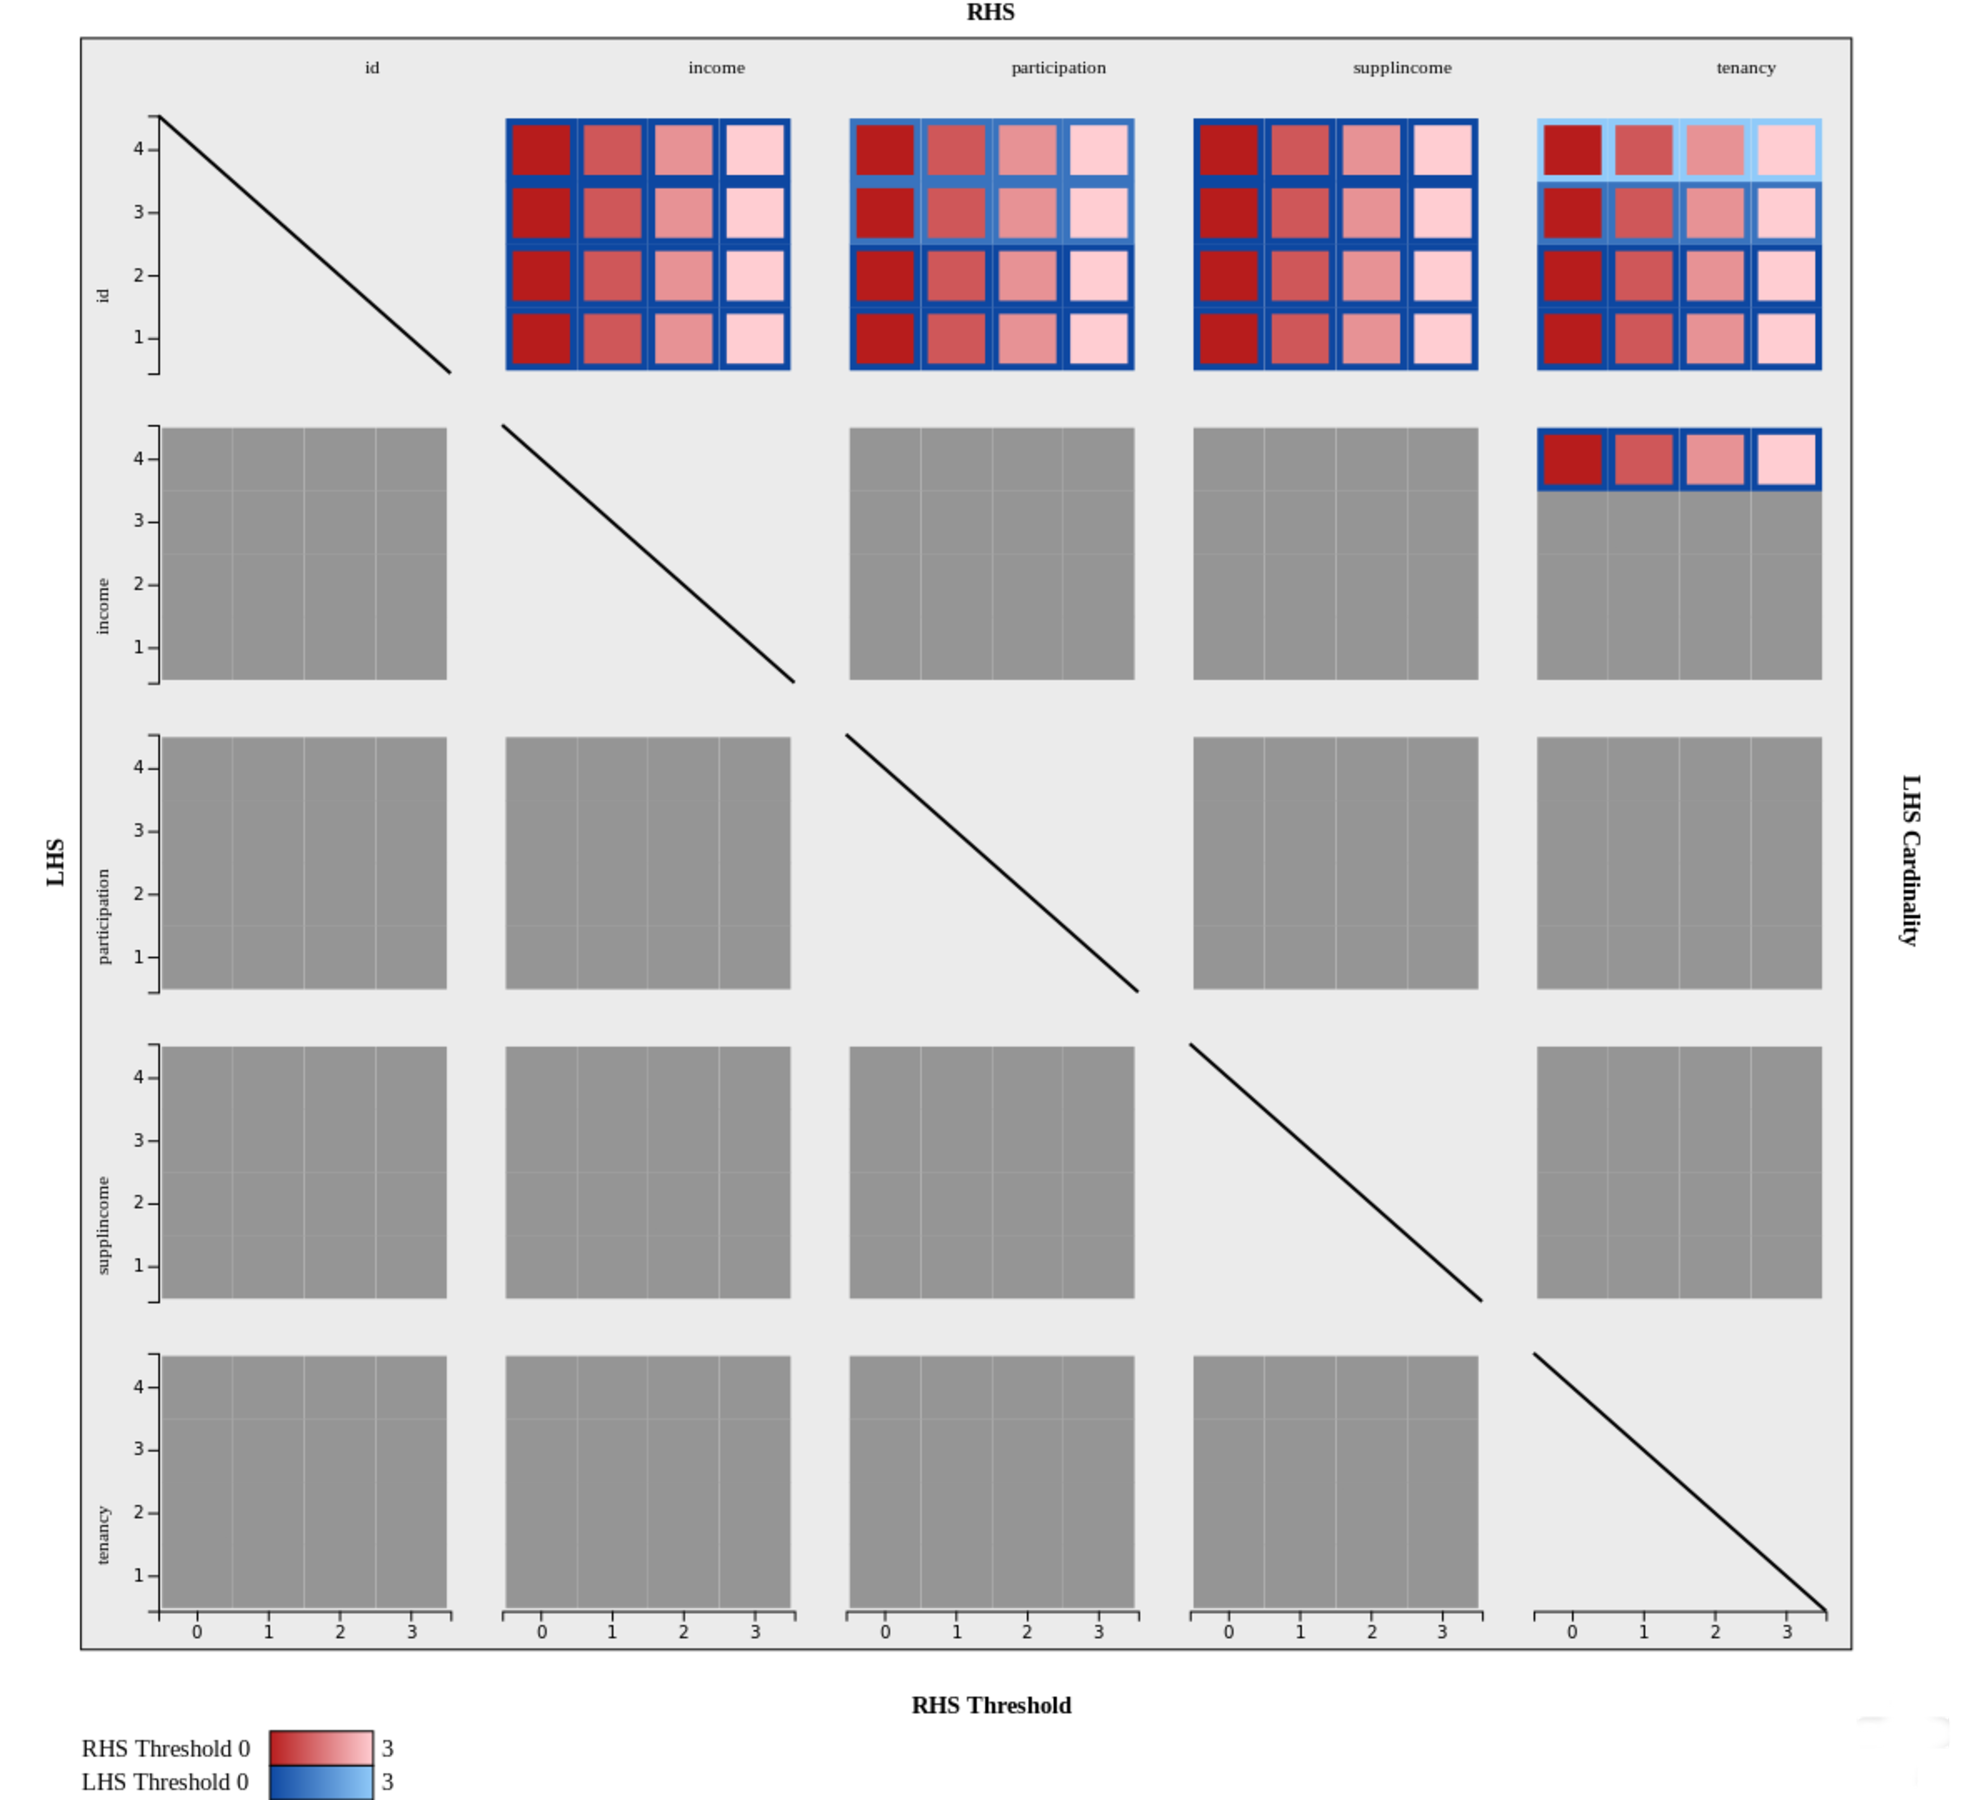
\includegraphics[width=\linewidth]{capitoli/figure/foodstamp_result}
    \caption{Rappresentazione ottenuta in output da Dependensee del dataset Foodstamp.}
    \label{fig:foodstamp_result}
\end{figure}
Consideriamo adesso il dataset \textit{Foodstamp}. La Figura \ref{fig:foodstamp_result} mostra la rappresentazione grafica ottenuta dando in input il dataset a Dependensee. Dal grafico ottenuto possiamo notare, attraverso la prima riga, come le uniche dipendenze esistenti siano con l'attributo \texttt{id} sul lato sinistro e, attraverso la seconda riga, con l'attributo \texttt{income} sul lato sinistro. Le prime sono in relazione con tutti gli altri attributi del dataset, infatti le colonne relative alla prima riga sono tutte colorate. Mentre, per l'attributo \texttt{income}, possiamo notare l'esistenza di \acrlong{rfds} solo con l'attributo \texttt{tenancy} sul lato destro. Le \acrlong{rfds} minimali presenti hanno quasi tutte una soglia minima o quasi, tranne quelle relative all'attributo \texttt{id} sul lato sinistro e l'attributo \texttt{tenancy} sul lato destro, le quali hanno soglia e cardinalit\`{a} massima. Con le righe e le colonne restanti possiamo notare che non vi sono \acrlong{rfds}, difatti sono colorate in grigio.\par
\begin{figure}[ht]
    \centering
    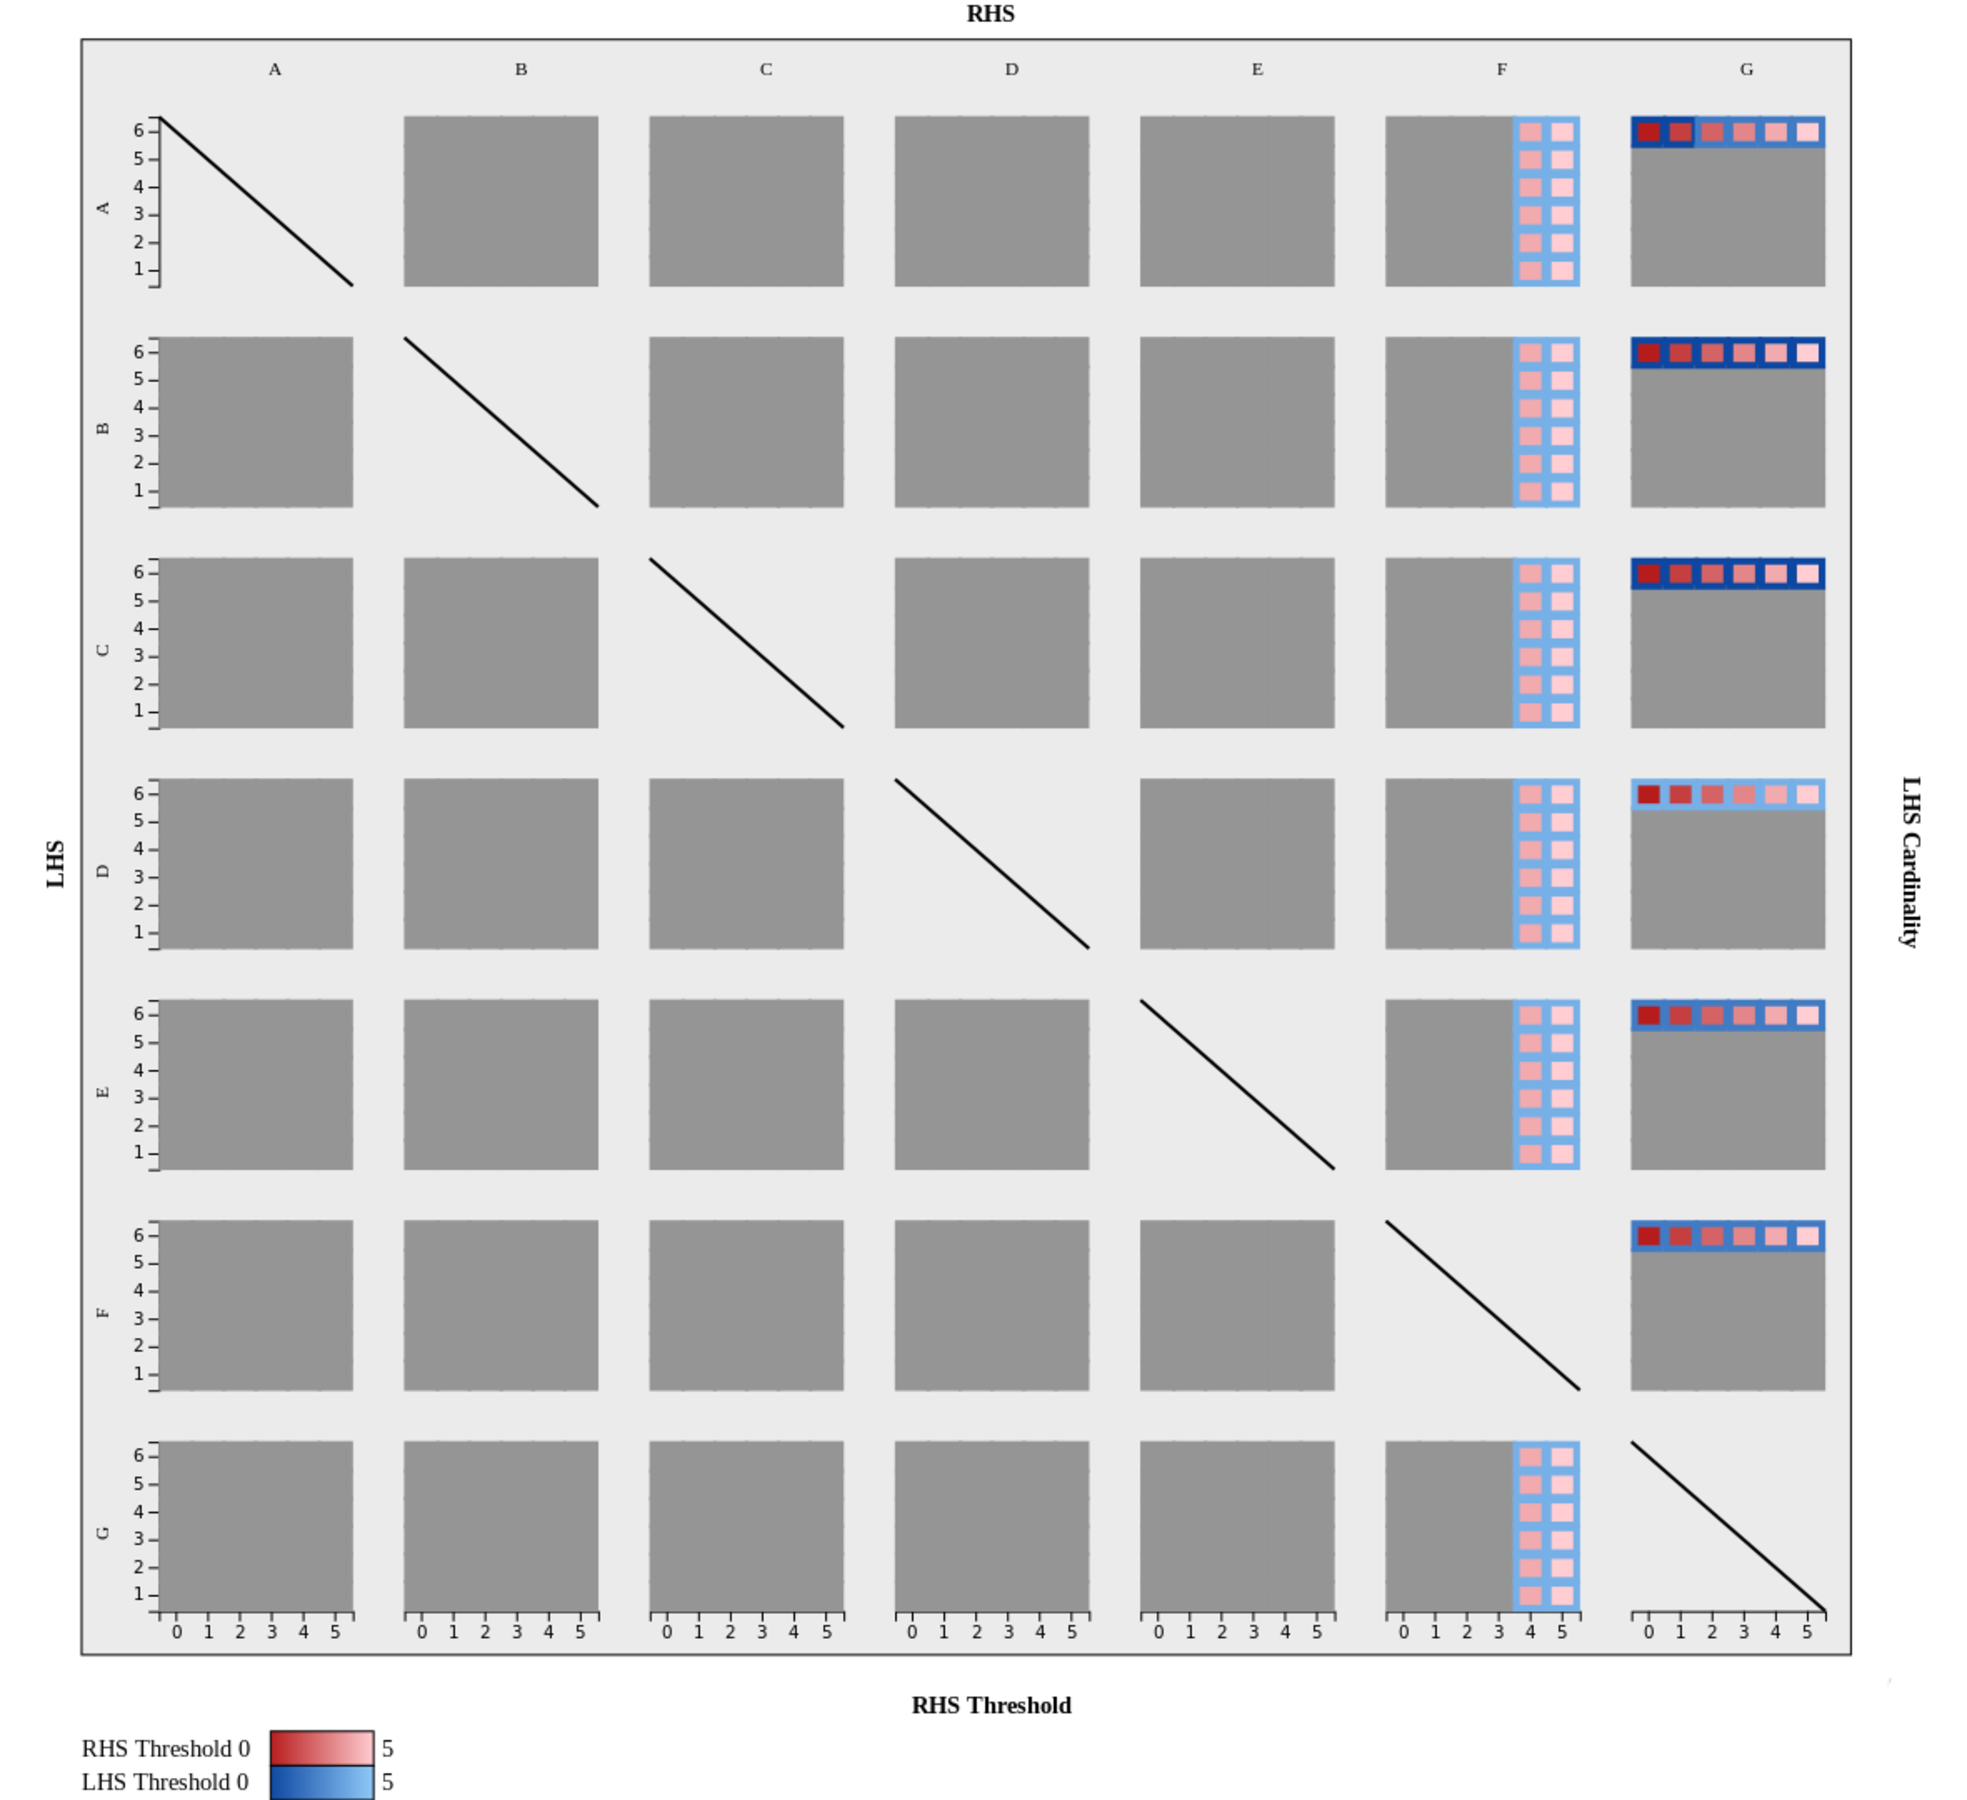
\includegraphics[width=\linewidth]{capitoli/figure/car_data}
    \caption{Rappresentazione ottenuta in output da Dependensee del dataset Car Data.}
    \label{fig:cardata_result}
\end{figure}
Il dataset \textit{Car\_Data} \`{e} stato analizzato con una soglia massima data in input pari a $5$. Le \acrlong{rfds} minimali presenti in questo dataset son poche e la maggior parte hanno una soglia alta. Se prendiamo in considerazione la colonna relativa all'attributo \texttt{F}, possiamo notare che le \acrlong{rfds} minimali esistenti siano tutte con una soglia sul lato sinistro pari a $5$ e soglia sul lato destro pari a $4$ e $5$. Se consideriamo, invece, la colonna relativa all'attributo \texttt{G}, possiamo notare che le \acrlong{rfds} minimali esistenti sono tutte con cardinalit\`{a} massima, con soglia massima o quasi sul lato sinistro e con soglia tra $0$ e $5$ sul lato destro.
\chapter{Conclusioni e Sviluppi futuri} %\label{1cap:spinta_laterale}
% [titolo ridotto se non ci dovesse stare] {titolo completo}
%
In questo capitolo verranno esposte le conclusioni relative al lavoro di tesi effettuato ed ai vari sviluppi futuri possibili del progetto di tesi.

\section{Conclusioni}
L'obiettivo di questa tesi \`{e} stato la realizzazione di un applicazione per la rappresentazione grafica di enormi insiemi di \acrlong{rfds} minimali, mediante l'utilizzo di una metafora di visualizzazione chiara ed immediata. L'applicazione deve interpretare un dataset di \acrshort{rfds} minimali e, successivamente, deve creare un grafico relativo al dataset analizzato. Quindi, la prima parte del lavoro di tesi si \`{e} esplorato il concetto di \acrlong{fd} e poi di \acrlong{rfd}, con un accenno agli algoritmi di ricerca delle \acrlong{rfds}. Tali informazioni sono state raccolte nel capitolo \ref{cap3:fd}. Dopo l'introduzione ai concetti appena citati, ci si \`{e} soffermati sulla rappresentazione grafica delle \acrlong{rfds}, introducendo il concetto di minimalit\`{a} delle \acrlong{fds} e \acrlong{rfds}, esplorando la metafora di visualizzazione proposta per la rappresentazione delle dipendenze \cite{mdvisualization}. Tali informazioni, invece, sono state raccolte nel capitolo \ref{cap4:visual_representation}. La terza ed ultima parte della tesi, descritta nel capitolo \ref{cap5:dependensee}, \`{e} stata dedicata allo sviluppo vero e proprio dell'applicazione ed alla successiva valutazione sperimentale. Questa ultima fase non ha presentato particolari problemi sulla rappresentazione grafica degli insiemi minimali, poich\'{e} i grafici sono creati dinamicamente. Durante la verifica sperimentale si \`{e} avuto modo di testare il corretto funzionamento dell'applicazione con l'utilizzo di diversi dataset. L'esito \`{e} stato positivo, la rappresentazione risultante per ogni dataset si \`{e} dimostrata efficace per analizzare visivamente tali dataset, in modo semplice ed efficace, riducendo di molto la difficolt\`{a} all'utente che la interpreta.

\section{Sviluppi futuri}
Un possibile sviluppo del progetto potrebbe essere la realizzazione di un'interfaccia grafica pi\`{u} gradevole, fornendo molte pi\`{u} informazioni e linee guida generali per guidare l'utente nell'utilizzo dell'applicazione. Inoltre, potrebbero essere implementate ulteriori funzioni che possano fornire informazioni pi\`{u} dettagliate. Ci\`{o} sarebbe possibile, ad esempio, tramite l'implementazione di ulteriori metafore di visualizzazione descritte in \cite{mdvisualization}, le quali forniscono informazioni pi\`{u} dettagliate riguardo le dipendenze di un determinato sottoinsieme del dataset. Infine, potrebbero essere previste delle applicazioni mobile per Android ed iOS, visto il grande utilizzo sempre pi\`{u} crescente degli smartphone e dei tablet in ambito lavorativo. Questo ulteriore sviluppo \`{e} facilitato dall'utilizzo di Ionic, il quale si propone come un Software Development Kit (SDK) per lo sviluppo non solo di applicazioni web, ma anche di applicazioni mobile ibride.

\newpage

%\part{Impatto ambientale}

\backmatter
%*******************************************************
% Bibliografia
%*******************************************************
\cleardoublepage
\phantomsection
\addcontentsline{toc}{chapter}{\bibname}
\nocite{*}
%\bibliographystyle{sample}
\bibliographystyle{plain}
%\bibliographystyle{plainnat}
\bibliography{bibliografia}
%

%\vspace{2.5cm}
%\begin{Large}Siti Web consultati\end{Large}
%\begin{itemize}
%\item Wikipedia -- \url{www.wikipedia.org}
%%\item -- \url{library.isgs.uiuc.edu}
%\end{itemize}


\phantomsection
\chapter{Ringraziamenti}
\markboth{Ringraziamenti}{}
% [titolo ridotto se non ci dovesse stare] {titolo completo}
% RINGRAZIAMENTI FINALI
Desidero innanzitutto ringraziare i miei relatori, il Prof. Vincenzo Deufemia e la Dott.ssa Loredana Caruccio, per la precisione e la disponibilit\`{a} mostratami durante il periodo di sviluppo del progetto e di stesura della tesi.\par
\vspace{5mm}
Dedico questo lavoro di tesi a mio padre e mia madre che hanno sempre creduto in me, supportandomi durante il mio percorso universitario. Un grazie particolare va a loro che, con il loro immancabile sostegno, mi hanno permesso di poter arrivare alla fine di questo percorso e senza tagliarmi i viveri.\par
\vspace{5mm}
Ringrazio Martina, la mia fidanzata, la quale ha vissuto con me parte di questo percorso, rimanendo al mio fianco. Lei mi ha sopportato e supportato nei momenti di gioia e debolezza e mi ha costantemente spronato.\par
\vspace{5mm}
Ringrazio i miei amici pi\`{u} cari per aver sempre creduto in me, per essermi stati vicini e per esserci sempre. Ringrazio, inoltre, i miei colleghi universitari con i quali ho condiviso questo percorso, tra cui quelli che ad oggi posso definire amici, che nel loro piccolo hanno contribuito a rendermi la persona che sono oggi.\par

\vfill
Grazie a tutti voi.
\end{document}
